\documentclass[12pt,a4paper,twoside,openright]{report}

\usepackage[utf8]{inputenc}
% \usepackage{csquotes}

\usepackage{lmodern}

\usepackage[romanian]{babel}
\addto\captionsromanian{%
  \renewcommand{\bibname}{Bibliografie}%
  \renewcommand{\appendixpagename}{Anexe}%
  \renewcommand{\lstlistingname}{Programul}%
}

% Dimensiunile paginii și margini
\usepackage{geometry}           
\geometry{
    a4paper,
    left=2.5cm,
    right=2.5cm,
    top=2.5cm,
    bottom=2.5cm,
}

\usepackage{lstautogobble}

\usepackage{setspace}
\onehalfspacing

\usepackage{parskip}

\usepackage[unicode]{hyperref}

\usepackage{biblatex}
\addbibresource{references.bib}

\usepackage{graphicx}
\graphicspath{ {./figures/} }
\usepackage{wrapfig}

\usepackage{multicol}
\usepackage{enumitem}
\setlist{nosep}

% Remove chapter numbering
% \makeatletter
% \def\@makechapterhead#1{%
%   \vspace*{50\p@}%
%   {\parindent \z@ \raggedright \normalfont
%     \interlinepenalty\@M
%     \Huge \bfseries #1\par\nobreak
%     \vskip 40\p@
%   }}
% \def\@makeschapterhead#1{%
%   \vspace*{50\p@}%
%   {\parindent \z@ \raggedright
%     \normalfont
%     \interlinepenalty\@M
%     \Huge \bfseries  #1\par\nobreak
%     \vskip 40\p@
%   }}
% \makeatother

% Code Blocks
\usepackage{listings}
\usepackage{color}


\definecolor{backcolour}{RGB}{242,242,242}
\definecolor{javared}{rgb}{0.6,0,0}
\definecolor{javagreen}{rgb}{0.25,0.5,0.35}
\definecolor{javapurple}{rgb}{0.5,0,0.35}
\definecolor{javadocblue}{rgb}{0.25,0.35,0.75}

\lstdefinestyle{javaCodeStyle}{
  language=Java,                         % the language of the code
  backgroundcolor=\color{backcolour},    % choose the background color; you must add \usepackage{color} or \usepackage{xcolor}
  basicstyle=\fontsize{10}{8}\sffamily,
  breakatwhitespace=false,
  breaklines=true,
  keywordstyle=\color{javapurple}\bfseries,
  stringstyle=\color{javared},
  commentstyle=\color{javagreen},
  morecomment=[s][\color{javadocblue}]{/**}{*/},
  captionpos=t,                          % sets the caption-position to bottom
  frame=single,                          % adds a frame around the code
  numbers=left,
  numbersep=10pt,                         % margin between number and code block
  keepspaces=true,                       % keeps spaces in text, useful for keeping indentation of code (possibly needs columns=flexible)
  columns=fullflexible,
  showspaces=false,                      % show spaces everywhere adding particular underscores; it overrides 'showstringspaces'
  showstringspaces=false,                % underline spaces within strings only
  showtabs=false,                        % show tabs within strings adding particular underscores
  tabsize=2                              % sets default tabsize to 2 spaces
}

\usepackage[toc,page]{appendix}
\usepackage{lipsum}
\usepackage{caption}
\usepackage{subcaption}

\author{\student}
\title{\fullTitle}
\date{2019\\ September}

\begin{document}

    \newcommand{\AppNameB}          {\textbf{ReceiptScan}}
\newcommand{\AppName}           {ReceiptScan}
\newcommand{\thesistitle}       {ReceiptScan}
\newcommand{\thesissubtitle}    {Aplicație Android pentru digitalizarea bonurilor fiscale}
\newcommand{\prof}              {prof. Ioana Leuștean}
\newcommand{\student}           {Lucian Boacă}
\newcommand{\session}           {septembrie, 2019}
\newcommand{\screenwidth}       {5cm}

    \begin{titlepage}
    \begin{center}
        \large
        \textbf{\MakeUppercase{Universitatea din București}}
        
        \textbf{\MakeUppercase{Facultatea de Matematică și Informatică}}
        
        \textbf{\MakeUppercase{Specializarea Informatică}}
        
        \vspace{3.5cm}
        
        \textbf{Lucrare de licență}
        
        \huge
        \textbf{\thesistitle}
        
        \large
        -\\
        \textbf{\thesissubtitle}
        
        \vspace{7.5cm}
        
        \begin{minipage}{7cm}
            \textbf{Coordonator științific}\\
            \textbf{\prof}
        \end{minipage}
        \hfill
        \begin{minipage}{3.3cm}
            \textbf{Absolvent}\\
            \textbf{\student}
        \end{minipage}
        
        \vfill
        \textbf{București, \session}
        
    \end{center}
\end{titlepage}


    \pagenumbering{gobble}

    \vspace*{\fill}

\begin{flushright}
  \textbf{\emph{Semnătura profesorului coordonator}}\\
  \dottedline
\end{flushright}

\vspace{1cm}
\begin{center}
  \large
  \textbf{Declarație}
\end{center}

Subsemnatul \student, candidat la examenul de \textbf{licență}, sesiunea \textbf{septembrie 2019}, la Universitatea din București, Facultatea de Matematică și Informatică, programul de studii Informatică, declar pe propria răspundere că lucrarea de față este rezultatul muncii mele, pe baza cercetărilor mele și pe baza informațiilor obținute din surse care au fost citate și indicate, conform normelor etice, în note și în bibliografie. Declar că nu am folosit în mod tacit sau ilegat munca altora și că nici o parte din teză nu încalcă drepturile de proprietate intelectuală ale altcuiva, persoană fizică sau juridică. Declar că lucrarea nu a mai fost prezentată sub această formă unei alte instituții de învățământ superior în vederea obținerii unui grad sau titlu științific ori didactic.

\vspace*{\fill}

\begin{flushright}
Semnătura,\\
\dottedline
\end{flushright}

\pagebreak

    \begin{center}
  \vspace*{\abstractTop}
  \huge
  \textbf{Abstract}
  \vspace*{\abstractBottom}
\end{center}

\normalsize
Urmărirea cheltuielilor este o sarcină importantă pentru a avea o viziune clară asupra situației financiare personale. Aplicațiile mobile existente rezolvă doar parțial această problemă. Acestea fie oferă prea puține informații, fie necesită un efort mult prea mare din partea utilizatorului. \AppName{} oferă o soluție pentru urmărirea cheltuielilor, facilitând scanarea chitanțelor de cumpărături și oferind datele extrase într-un mod flexibil.

Pentru rezolvarea problemei am dezvoltat această aplicație Android ce utilizează un modul OCR avansat și un set de reguli pentru a extrage informații din bonuri fiscale. Aceasta pune la dispoziția utilizatorului un eran de vizualizare a cheltuielilor sale și opțiunea de a exporta datele în cloud pentru a le descărca apoi în afara dispozitivului.

La momentul scrierii și din căutările făcute, aceasta este o abordare unică. Aplicația este disponibilă în mod open source, pe GitHub. Aceasta oferă rezultate suficient de bune și poate fi ușor extinsă cu alte reguli pentru diferite tipuri chitanțe.

\clearpage
    \begin{center}
  \vspace*{\abstractTop}
  \huge
  \textbf{Abstract}
  \vspace*{\abstractBottom}
\end{center}

\normalsize

Expenses tracking is an important task for having a clear view over personal financial situation. Existing mobile apps solve this problem only partially. They either offer way to few information or require a great involvement on the user side. \AppName{} offers a solution for expenses tracking, making it easy to scan receipts and offering the extracted data in a flexible way.

For solving this problem, I developed this Android app which makes use of an advanced OCR module and a set of rules to extract the information out of receipts. This app displays a repports screen to show user's spending and offers the option to export the data in cloud to further be downloaded outside the device.

At the moment of writing and from the my research, this is an unique approach. The app is available open source on GitHub. It offers good enough results and it can easily be extended with other rules for different receipt types.

\clearpage


    \tableofcontents
  
    \listoffigures

    \chapter{Introducere}\label{introducere}
\pagenumbering{arabic}
\setcounter{page}{1}

Această lucrare prezintă \AppNameB, o aplicație mobilă de scanare a bonurilor fiscale și vizualizare a cheltuielilor, disponibilă pentru platforma \emph{Android}.

% \section{Motivație}

Urmărirea și analizarea cheltuielilor este o sarcină importantă pentru alcătuirea unui buget personal și pentru o organizare mai bună a activităților financiare. Popularizarea în ultimii ani a plăților electronice și cu cardul a facilitat apariția a tot mai multe astfel de servicii automate. Majoritatea băncilor oferă astăzi o aplicație mobilă cu funcționalitatea de a urmări și clasifica tranzacțiile clienților.

Cea mai mare problemă pe care aceste servicii o întâmpină este lipsa unor date mai bogate, fără de care valoarea pe care o pot aduce este limitată. Într-adevăr, soluțiile existente valorifică un set limitat de date disponibile tranzacțiilor, printre care numele comerciantului și suma totală. Fără a avea acces la conținutul tranzacției, serviciile existente nu pot oferi o listă comprehensivă cu toate achizițiile utilizatorului.

O altă problemă a serviciilor oferite de bănci pentru urmărirea cheltuielilor este disponibilitatea datelor. Utilizatorii au acces limitat la datele ce le aparțin. Aceste date sunt disponibile fie doar în aplicația băncii, fie pot fi exportate în formate ce nu pot fi valorificate mai departe, cum ar fi documente PDF. În acest caz, o întrebare simplă, cum ar fi \textit{Cât am cheltuit în această lună pe pâine?} devine greu de răspuns.

Având în vedere dezavantajele soluțiilor curente, am dezvoltat \AppName, o aplicație care să ofere o mai mare vizibilitate asupra tranzacțiilor financiare. Aceasta permite scanarea bonurilor fiscale, înțelegerea automată a acestora, prezentarea grafică și stocarea acestora într-o bază de date locală și exportul acestora în cloud, de unde pot fi descărcate pentru o analiză mai amănunțită utilizând uneltele utilizatorului.

% \section{Obiective}

În procesul de dezvoltare a aplicației \AppName{} mi-am propus:
\begin{enumerate}
  \item 
  \textbf{Dezvoltarea și îmbunătățirea algoritmului de extragere de informații}: Extragerea informațiilor structurate din imagini este un proces complex, ce nu poate avea o soluție standard, care să funcționeze în orice caz. În plus, lipsa unei metode formale de evaluare a sarcinii de înțelegere a conținutului chitanțelor din imagini acceptată la scară largă îngreunează dezvoltarea de noi metode. Acest proiect aplică un set de metode euristice, cu scopul de a înțelege o gamă cât mai largă de bonuri fiscale populare în România și de a necesita un efort minim din partea utilizatorului;
  \item
  \textbf{Valorificarea confidențialității utilizatorului}: Datele financiare ale utilizatorilor pot fi fructificate de către agenții de publicitate din mediul online și de aceea utilizatorii pot fi reticenți în a folosi o aplicație care are acces la acestea. Am gândit această aplicație astfel încât comunicarea cu un server să se facă doar voluntar și complet anonim, astfel încât informațiile despre achiziții să nu poată fi legate de un anumit utilizator;
  \item
  \textbf{Implementarea unor standarde înalte ale structurii codului}: Calitatea codului și organizarea acestuia au un puternic impact asupra succesului unui proiect software pe termen mediu și lung. În cadrul acestui proiect mi-am propus explorarea bunelor practici în dezvoltarea aplicațiilor \emph{Android} și construirea unei arhitecturi care să faciliteze testarea și decuplarea sistemului și care să fie ușor de înțeles și implementat.
\end{enumerate}

% \section{Lucrări asemănătoare}\label{related_intro}

Analizarea și procesarea chitanțelor financiare pe baza imaginilor obținute folosind camera foto a telefoanelor a stârnit un interes moderat în comunitatea științifică și tehnică. \emph{Janssen et al.} prezintă în lucrarea \emph{Receipts2Go} \cite{Receipts2Go} o abordare bazată pe OCR și expresii regulate pentru a extrage datele despre tranzacții, dar nu include lista de produse. \emph{Raoui-Outach et al.} prezintă în lucrarea \emph{Deep Learning for automatic sale receipt understanding} \cite{DL_receipt_understanding} o abordare de procesare bazată pe \emph{deep learning}.

% \section{Structura lucrării}\label{structura_intro}

Această lucrare este structurată după cum urmează. Capitolul \ref{specs} prezintă specificațiile aplicației \AppName într-un mod semi-formal. Capitolul \ref{technical} motivează platforma aleasă și descrie tehnologiile folosite, arhitectura aplicației și detaliile de persistență. În capitolul \ref{implementation} sunt prezentate detaliile de implementare și provocările tehnice întâmpinate. Lucrarea se încheie în capitolul \ref{conclusions} prin prezentarea concluziilor și a observațiilor de final.

    \chapter{Specificațiile aplicației}\label{specs}

În cadrul dezvoltării unui produs software, definirea specificațiilor are un rol crucial în succesul proiectului. Această etapă poate implica studii laborioase de piață, iar specificațiile pot trece prin mai multe etape, de la discuții cu utilizatorii până la documente formale ce ajung la programatori. În cazul de față, specificațiile sunt dictate de nevoile personale și pot fi formulate într-un limbaj mai apropiat de cel tehnic, gata de implementare.

Specificațiile sunt definite în jurul noțiunii de \emph{usecase} (caz de utilizare), așa cum acestea sunt definite în lucrarea \emph{Structuring use cases with goals} \cite{cockburn1997structuring} și inspirate din exemplul prezentat în \emph{The Pragmatic Programmer} \cite{Hunt:2000:PPJ:320326}. Așadar, \textbf{scopul} acestor \emph{usecases} este de a defini specificațiile, \textbf{conținutul} este proza consistentă (descriere în cuvinte astfel încât să nu apară contradicții), \textbf{pluralitatea} este de unul sau mai multe scenarii per \emph{usecase}, iar \textbf{structura} este semi-formală.

În continuare este prezentat fiecare caz de utilizare astfel: o scurtă descriere a funcționalității însoțită de \emph{screenshot-uri} din aplicație, acolo unde sunt necesare care este urmată de o prezentare schematică. Această schemă dă structura în care este implementată funcționalitatea și ajută la definirea testelor. Din punct de vedere al terminologiei, \textbf{mențiunile} dau detalii și cerințe non-funcționale, \textbf{principalul scenariu} descrie pașii necesari pentru realizarea scopului, \textbf{variațiile} definesc puncte ce pot fi implementate în moduri multiple, cum ar fi mai multe surse de date și care sunt relevante pentru scop, iar \textbf{extensiile} sunt scenarii secundare, ce servesc scopul principal.

\section{Capturarea și înțelegerea imaginilor}\label{understanding_spec}

% \begin{wrapfigure}{R}{0.3\textwidth}
%   \centering
%   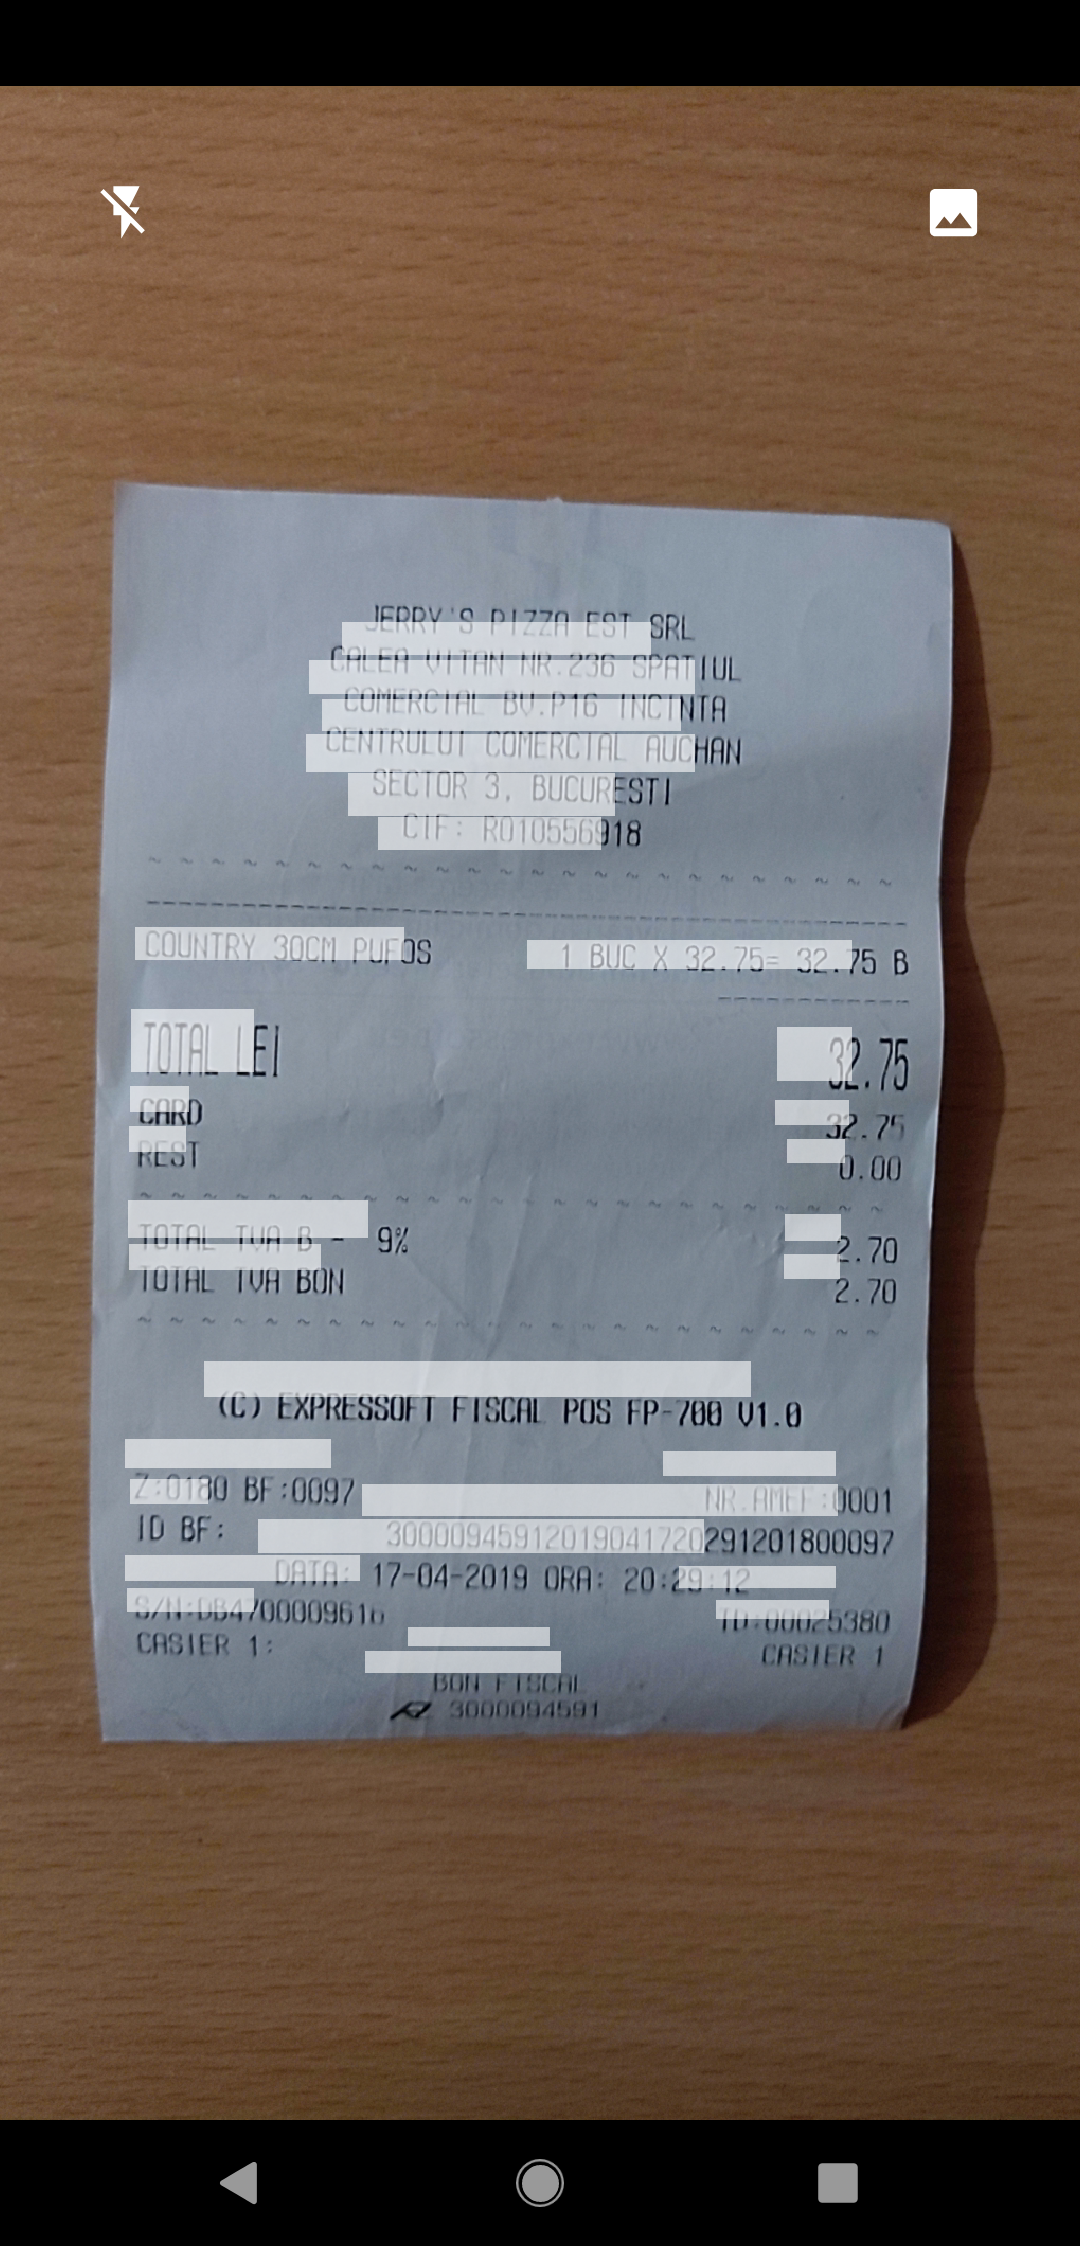
\includegraphics[width=0.25\textwidth]{Scanner.png}
%   \caption{Ecranul de Scanare}
%   \label{fig:scanner}
% \end{wrapfigure}
% \lipsum[1]


Aceasta este principala funcționalitate a aplicației și are ca scop extragerea informațiilor despre tranzacție dintr-o imagine cu un bon fiscal. Interfața cu utilizatorul este reprezentată de un vizor pentru camera principală a dispozitivului, ce afișează în timp real si textul detectat în imagine în spatele unor chenare.  Capturarea imaginii se face prin gestul \emph{tap} pe ecran. Funcționalitatea permite și folosirea unei imagini din galerie, dar și folosirea \emph{flash-ului} în condițiile de iluminare slabă. Odată capturată o imagine, procesarea acesteia se face pe un \emph{thread} secundar, în timp ce un ecran de încărcare este afișat. Figura \ref{fig:scanner} prezintă ecranul de scanare și chenarele de text recunoscute în imagine.

\begin{figure}[ht]
  \centering
  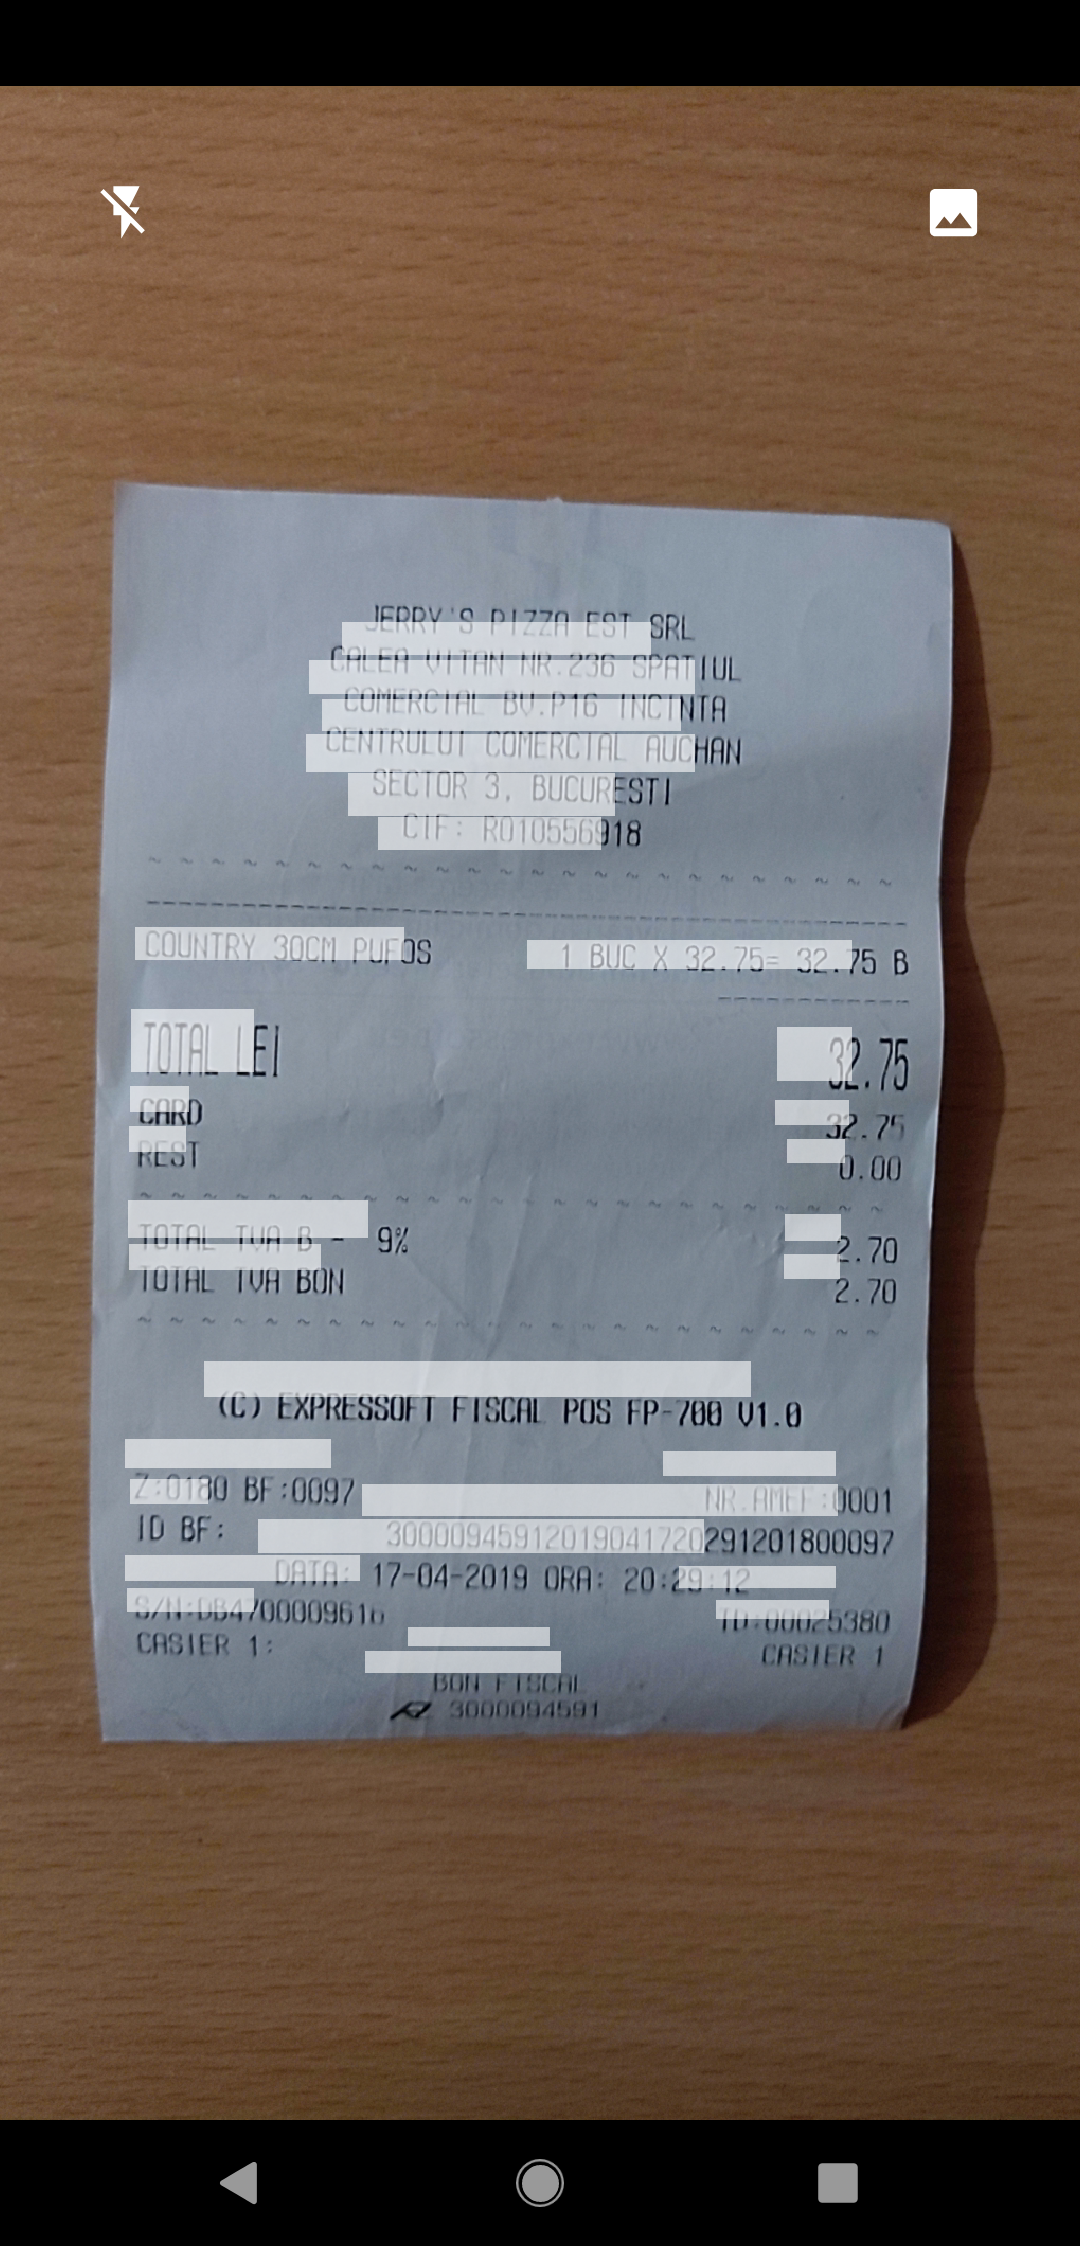
\includegraphics[width=\screenwidth]{Scanner.png}
  \caption{Ecranul de Scanare}
  \label{fig:scanner}
\end{figure}

\begin{itemize}
\item
  \textbf{Scop}: Capturarea unei imagini și extragerea informațiilor relevante din aceasta;
\item
  \textbf{Condiție de succes}: Prezența unei înregistrări în baza de date ce modelează bonul fiscal în starea de \emph{draft};
\item
  \textbf{Condiții de eșec}: Imaginea nu poate fi capturată; modulul OCR nu funcționează; o imagine este deja în curs de procesare;
\item
  \textbf{Precondiții}: Valorile predefinite pentru categorie și monedă;
\end{itemize}

\subsection*{Mențiuni}

Informațiile relevante de extras dintr-o imagine sunt:
\begin{multicols}{3}
\begin{itemize}
\item
  nume comerciant;
\item
  data tranzacției;
\item
  suma totală;
\item
  moneda;
\item
  categoria tranzacției;
\item
  produse:
  \begin{itemize}
  \item
    numele produsului;
  \item
    prețul aferent;
  \end{itemize}
\item
  elementele OCR:
  \begin{itemize}
  \item
    coordonatele casetelor de text;
  \item
    textul aferent;
  \end{itemize}
\end{itemize}
\end{multicols}

Imaginile se salvează astfel încât să nu fie accesibile din galerie.

\subsection*{Principalul scenariu}\label{principalul-scenariu}

\begin{enumerate}
\item
  Utilizatorul capturează o imagine;
\item
  Modulul OCR este apelat; Textul și chenarele aferente sunt extrase;
\item
  Rezultatul OCR este procesat pentru a obține conținutul bonului;
\item
  Bonul fiscal este salvat în stadiu de draft pentru a fi editat;
  (Specificație \ref{editare-draft})
\end{enumerate}

\begin{minipage}[t]{0.39\textwidth}
  \subsection*{Variații}\label{variaux21bii}
  \begin{itemize}
  \item
    Imaginea poate fi capturată utilizând camera telefonului sau importată
    din galerie;
  \item
    Moneda și categoria pot avea valori prestabilite, ce se modifică din setări; (Specificație \ref{spec:setari})
  \end{itemize}
\end{minipage}
\hspace{0.01\textwidth}
\begin{minipage}[t]{0.6\textwidth}
  \subsection*{Extensii}\label{extensii}
  \begin{itemize}
  \item
    Pentru a ajuta utilizatorul atunci când folosește camera, procesarea
    imaginilor venite de la cameră se face continuu, la o rată maximă
    configurabilă;
  \item
    Nu pot fi procesate mai multe imagini în același timp. Starea ultimei
    procesări este accesibilă permanent. Dacă se primește o cerere de
    procesare înainte ca ultima să se fi încheiat este semnalată o eroare.
  \end{itemize}
\end{minipage}


\section{Editare draft}\label{editare-draft}

Întrucât extragerea informațiilor nu este un proces robust, datele extrase trebuie validate de utilizator. Odată ce imaginile sunt procesate, datele extrase sunt salvate în baza de date, sub categoria \emph{drafts}. În acest moment, bonurile sunt editabile. Figura \ref{fig:draftList} prezintă ecranul unde utilizatorul vede toate drafturile, iar figura \ref{fig:draftScreen} ilustrează ecranul de editare.

\begin{figure}[!ht]
  \centering
  \begin{subfigure}{0.49\textwidth}
    \centering
    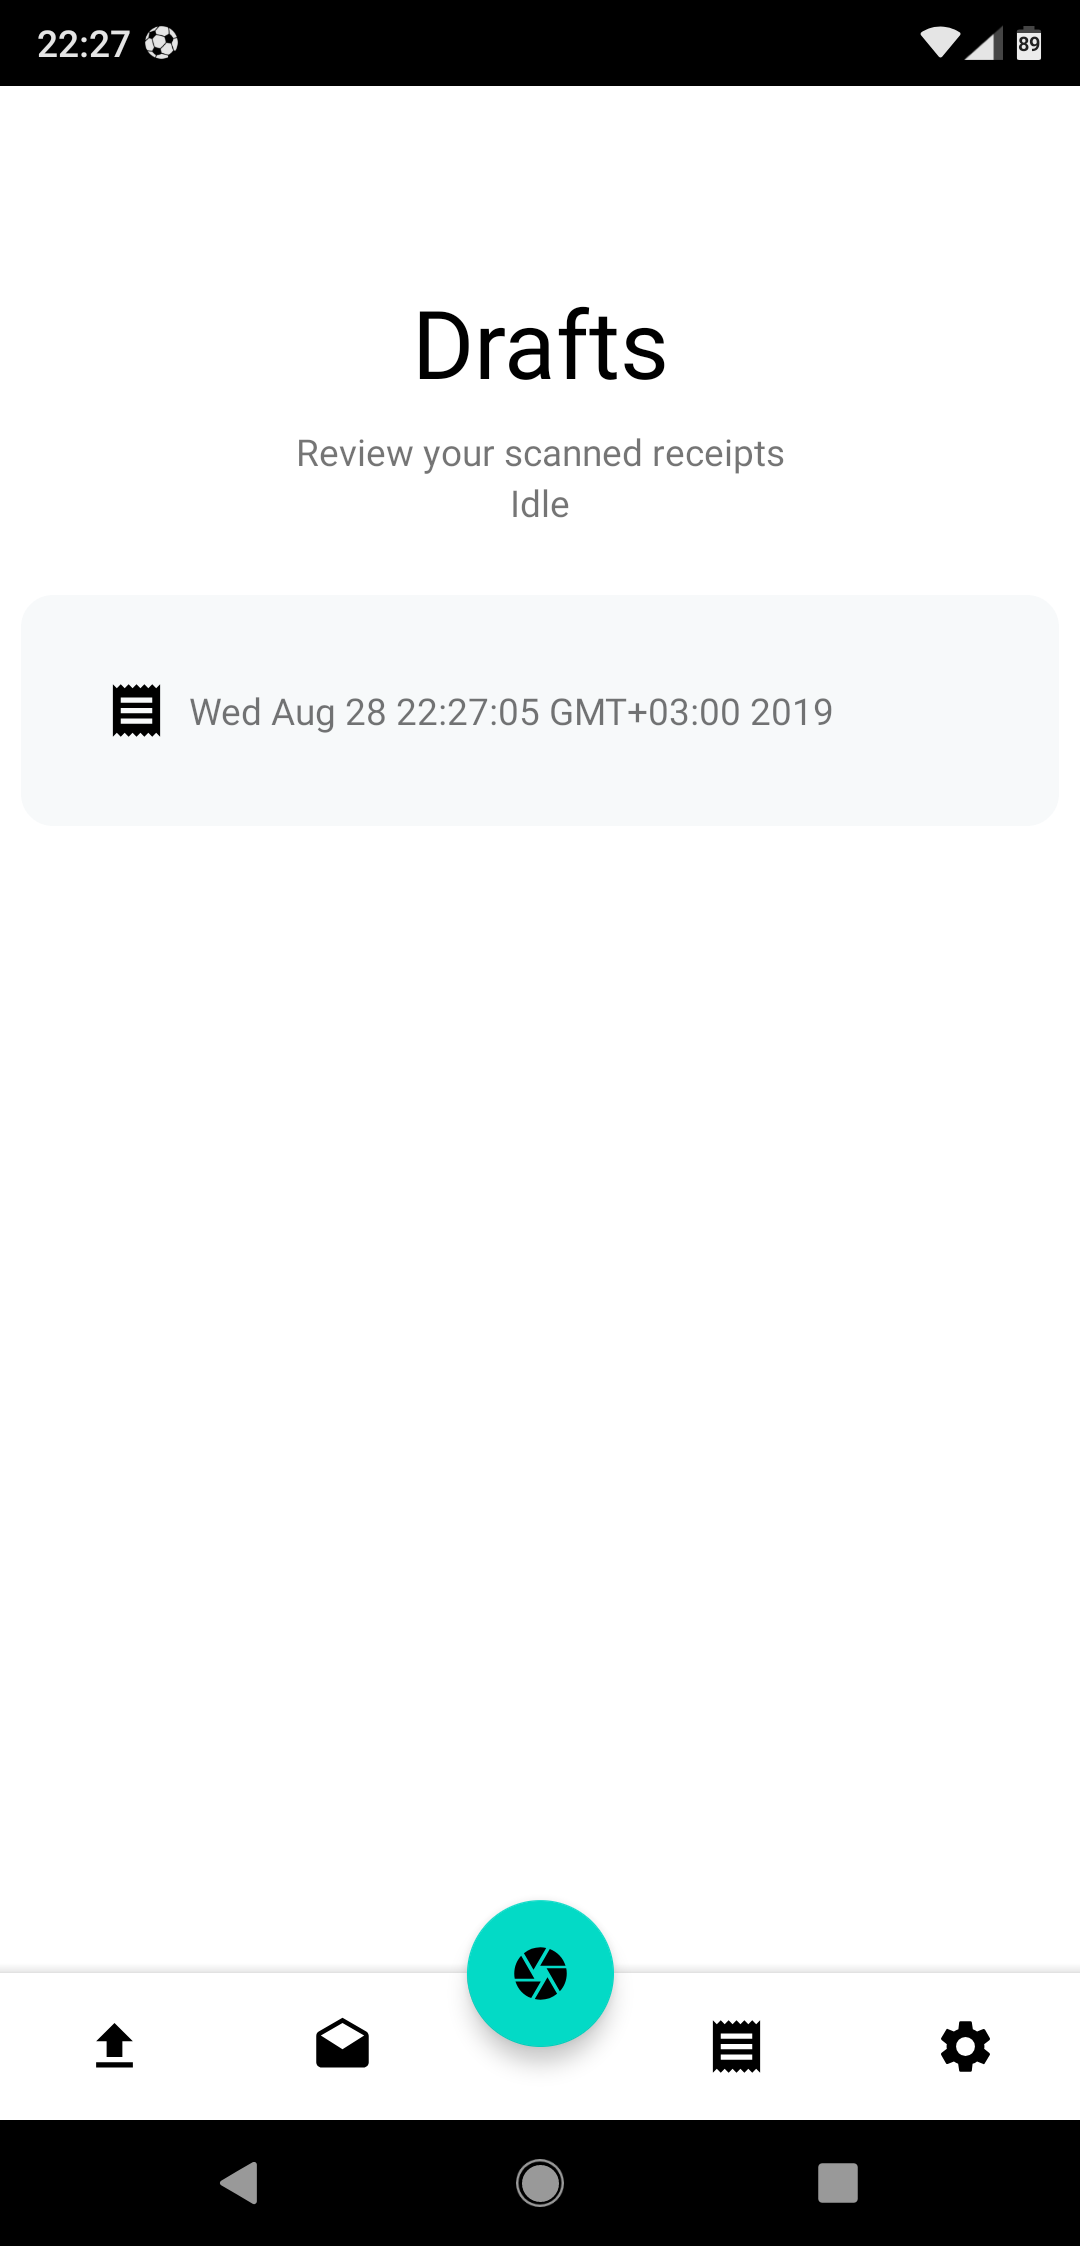
\includegraphics[width=\screenwidth]{DraftsList.png}
    \caption{Ecranul de listare}
    \label{fig:draftList}
  \end{subfigure}
  \begin{subfigure}{0.49\textwidth}
    \centering
    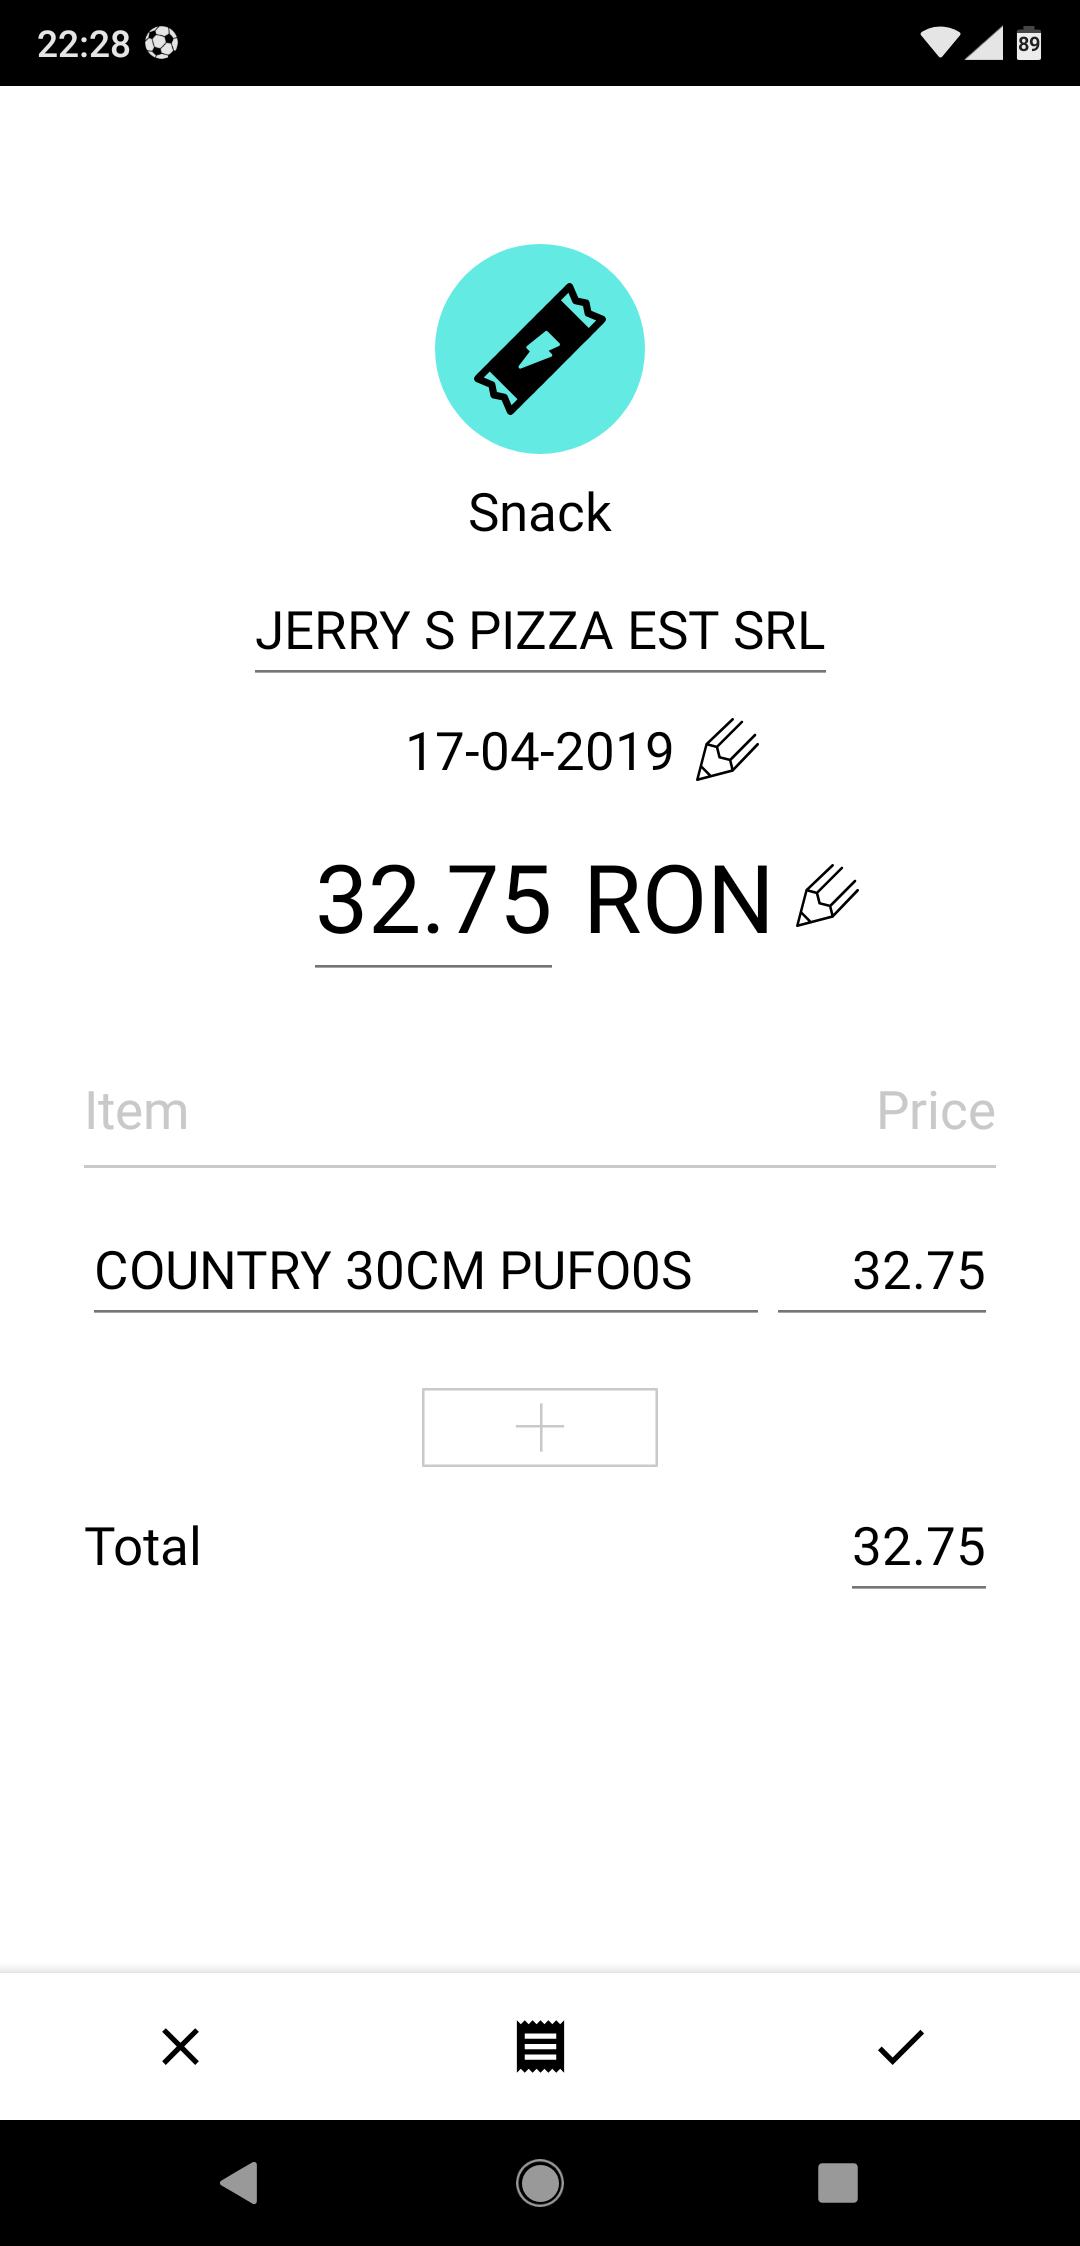
\includegraphics[width=\screenwidth]{DraftScreen.png}
    \caption{Ecranul de editare}
    \label{fig:draftScreen}
  \end{subfigure}
  \caption{Ecranele de gestionare a drafturilor}
  \label{fig:drafts}
\end{figure}

\begin{itemize}
\item
  \textbf{Scop}: Validarea informațiilor extrase din imagine de către utilizator;
\item
  \textbf{Condiție de succes}: Modificările făcute de utilizator se reflectă în baza de date; Bonul este validat și marcat ca final;
\item
  \textbf{Condiții de eșec}: Modificările nu pot fi persistate; Modificările sunt invalide;
\end{itemize}

\subsection*{Mențiuni}

Algoritmul de validare poate fi subiectul unor modificări ulterioare și trebuie să fie ușor de înlocuit.

Validarea considerată la momentul scrierii presupune ca niciun câmp să nu fie null sau fără conținut.

Asupra unui draft, utilizatorul are la dispoziție următoarele opțiuni:
\begin{multicols}{2}
\begin{itemize}
  \item
    modificarea categoriei, prin apăsarea pe ilustrația corespunzătoare;
  \item
    modificarea numelui comerciantului;
  \item
    modificarea datei, prin folosirea unui \emph{date picker};
  \item
    modificarea prețului total și a monedei;
  \item
    modificarea numelui sau prețului unui produs;
  \item
    ștergerea unui produs, prin gestul de \emph{swipe};
  \item
    adăugarea unui produs, prin apăsarea butonului de adăugare;
  \item
    ștergerea sau validarea \emph{draft-ului} și vizualizarea imaginii aferente prin butoanele din bara de opțiuni;
\end{itemize}
\end{multicols}

\subsection*{Principalul scenariu}


% \begin{minsipage}[t]{0.55\textwidth}

\begin{enumerate}
\item
  Utilizatorul accesează un bon;
\item
  Utilizatorul modifică câmpurile dorite;
\item
  Utilizatorul cere validarea bonului; Validarea se efectuează cu succes;
\item
  Bonul este scos din lista \emph{drafts} și pus în lista bonurilor validate;
\end{enumerate}

% \end{minipage} \vspace{0.01\textwidth}
% \begin{minipage}[t]{0.44\textwidth}

\subsection*{Variații}

\begin{itemize}
\item
  Utilizatorul poate modifica valori, dar fără a valida bonul;
\item
  Utilizatorul poate valida bonul, ceea ce îl scoate din lista de \emph{drafts} și îl pune în lista de bonuri valide;
\item
  Accesarea unui bon se face fie prin alegerea acestuia din listă, fie în urma scanării unei imagini; (Înțelegerea imaginilor)
\end{itemize}
% \end{minipage}
  
\subsection*{Extensii}

\begin{itemize}
\item
  Utilizatorul poate vedea imaginea capturată, cu și fără elementele OCR;
\item
  Utilizatorul poate vedea toate bonurile din lista \emph{drafts} și poate naviga către unul din ele;
\end{itemize}




\section{Gestionare setări}\label{spec:setari}

\begin{itemize}
\item
  \textbf{Scop}: Modificarea și accesarea unor valori folosite în diferite puncte ale aplicației;
\item
  \textbf{Scenariu de succes}: Modificările făcute de utilizator sunt persistate și pot fi accesate;
\item
  \textbf{Scenarii de eșec}: Modificările nu pot fi persistate; Valorile nu pot fi accesate;
\end{itemize}

Setările considerate sunt:

\begin{itemize}
\item
  Valoarea predefinită pentru categorie;
\item
  Valoarea predefinită pentru monedă;
\item
  Activarea sau dezactivarea colectării anonime de date;
\end{itemize}

\subsection{Principalul scenariu}\label{principalul-scenariu-2}

\begin{enumerate}
\item
  Utilizatorul accesează setările
\item
  Utilizatorul modifică valoarea unei setări;
\item
  Noua valoare este persitată și accesibilă;
\end{enumerate}

\section{Colectare bonuri fiscale}\label{colectare-bonuri-fiscale}

\begin{itemize}
\item
  \textbf{Scop}: Utilizatorul salvează un bon, acesta este sincronizat în cloud numai dacă utilizatorul permite colectarea de date;
\item
  \textbf{Condiție de succes}: Bonul este trimis cu succes către server;
\item
  \textbf{Condiții de eșec}: Colectarea este permisă, utilizatorul salvează un bon, acesta nu este sincronizat în cloud; Datele nu pot fi accesate la momentul sincronizării;
\item
  \textbf{Precondiții}: Colectarea este permisă sau nu
\end{itemize}

\subsection{Mențiuni}\label{menux21biuni-2}

Acțiunea de sincronizare se face în background, fără ca atenția utilizatorului să fie atrasă. Sincronizarea se face numai pe conexiune Wi-Fi și poate fi amânată până când conexiunea este disponibilă.

Se sincronizează toate informațiile aferente bonului, inclusiv imaginea și elementele OCR.

\subsection{Principalul scenariu}\label{principalul-scenariu-3}

\begin{enumerate}
\item
  Utilizatorul finalizează salvarea unui bon cu succes;
\item
  În consecința acțiunii de salvare, precondiția este interogată;
\item
  Dacă este permisă colectarea, bonul este sincronizat în cloud;
\end{enumerate}

\section{Export}\label{export}

\begin{itemize}
\item
  \textbf{Scop}: Accesarea datelor în afara aplicației și a dispozitivului;
\item
  \textbf{Condiție de succes}: Utilizatorul selectează formatul, conținutul și perioada pentru export și primește un link la care poate accesa datele;
\item
  \textbf{Condiție de eșec}: Nu există date înregistrate în perioada selectată; Datele nu sunt trimise cu succes; Utilizatorul nu primește link-ul aferent;
\end{itemize}

\subsection{Mențiuni}\label{menux21biuni-3}

Pentru a consuma cât mai puține resurse (timp, baterie), exportul se face cu minim de procesare pe dispozitiv;

Datele salvate pe cloud au o dată de expirare, după care sunt șterse;

Odată ce datele sunt încărcate și procesate în cloud, aplicația primește o notificare ce conține link-ul de descărcare;

Datele pot fi descărcate într-o arhivă zip;

\subsection{Variații}\label{variaux21bii-2}

\begin{itemize}
\item
  Pentru a oferi maximum de flexibilitate utilizatorilor, datele pot fi accesate in format JSON sau CSV și pot conține fie doar text, fie text și imagini;
\end{itemize}

\subsection{Extensii}\label{extensii-2}

\begin{itemize}
\item
  În cazul lipsei de conectivitate, acțiunea de export este programată pentru o dată ulterioară, odată ce telefonul are conexiune;
\item
  Toate sesiunile de export sunt înregistrare într-o listă și sunt eliminate odată ce datele aferente sunt șterse din cloud;
\end{itemize}

    \chapter{Tehnologii. Arhitectură. Persistență}\label{technical}

Un scop secundar al acestui proiect este explorarea unor metode moderne pentru dezvoltarea aplicațiilor Android. Menținerea unor reguli și structuri clare în organizarea codului aplicației aduce o serie de beneficii, printre care reducerea numărului de bug-uri și ușurința în menținerea și extinderea aplicației pe termen lung și este crucială pentru succesul proiectelor de dimensiuni medii și mari sau la care lucrează mai multe persoane. Dezavantajul acestora este timpul ce trebuie investit la începutul proiectului și o continuă disciplină și atenție din partea programatorilor.

\section{Alegerea platformei Android}

Decizia de a dezvolta această aplicație pentru platforma Android este susținută de motive atât tehnologice, cât și de oportunitate. Conform StatCounter, în Iulie 2019, sistemul de operare Android deținea 76.08\% cotă de piață la nivel global \cite{StatsWorldwide}, 73.71\% la nivelul Europei \cite{StatsEurope} și 81.3\% la nivelul României \cite{StatsRomania}. Aceste cifre justifică prioritizarea platformei Android în dezvoltarea unei aplicații mobile.

Din punct de vedere tehnologic, opțiunile pentru dezvoltarea unei aplicații mobile în 2019 sunt \emph{Android Nativ}, \emph{iOS Nativ} sau \emph{cross-platform}, folosind una dintre cele câteva soluții populare pentru dezvoltare cross-platform (printre care \emph{React Native}, \emph{Flutter} sau \emph{Native Script}). Nevoile tehnice ale acestei aplicații presupun integrarea unei soluții OCR, iar procesarea să se facă pe dispozitiv. Implementarea unei astfel de soluții într-un framework cross-platform nu este o sarcină trivială datorită lipsei de suport și documentație. Alegând între \emph{Android Nativ} și \emph{iOS Nativ}, dezvoltarea pentru Android se poate face de pe orice sistem de operare major, pe când dezvoltarea pentru iOS necesită sistemul de operare macOs. 

Analizând cele două motive de mai sus, am ales \emph{Android Nativ} ca platformă de dezvoltare datorită popularității sistemului de operare, a stabilității ecosistemului de dezvoltare și a suportului și a documentației extensive disponibile. Pentru o viitoare migrare către \emph{iOS}, framework-ul \emph{Flutter} este considerat ca fiind o soluție viabilă.

\section{Tehnologii utilizate}

Dezvoltarea pe platforma \emph{Android Nativ} oferă acces la întreg ecosistemul \emph{JVM}. Acest lucru a permis utilizarea a mai multor librării care nu au fost dezvoltate special pentru Android. În continuare vor fi prezentate tehnologiile folosite în dezvoltarea aplicației și motivația din spatele lor.

\subsection{Kotlin}

Dezvoltarea aplicațiilor Android nu mai înseamnă doar \emph{Java}. \emph{Kotlin} este un limbaj de programare ce rezolvă multe dintre problemele din Java și care, începând din 2017 este suportat în mod oficial de către \emph{Google} ca limbaj de dezvoltare pentru Android, iar din 2019, considerat limbaj preferat pentru Android. Aceasta înseamnă că noile funcționalități ale SDK-ului Android vor fi dezvoltate și oferite cu prioritate către \emph{Kotlin}.

Principalele caracteristici ale acestui limbaj sunt sistemul de tipuri superior, ce suportă inferența tipurilor, existența tipurilor de date care nu pot fi nule (\emph{null safety}), lipsa excepțiilor \emph{verificate} (\emph{checked exceptions}) și diferențierea clară și ușoară între variabile și constante (prin cuvintele cheie \texttt{var} și \texttt{val}). Codul scris în \emph{Kotlin} este de cele mai multe ori mai scurt, mai concis, mai sigur și mai ușor de înțeles decât cel scris în Java.

\subsection{RxJava}

\emph{Programare reactivă} \cite{ReactiveProgramming} este o paradigmă concentrată în jurul reacționării la modificări în starea unui obiect și a devenit populară în ultimii ani, atât pentru dezvoltarea aplicațiilor grafice, cât și pentru aplicațiile de server care procesează fluxuri de date. Avantajele acesteia sunt facilitarea procesării pe mai multe \emph{thread-uri} și abstractizarea componentelor aplicației (\emph{separation of concerns}).

RxJava implementează o serie de abstractizări ce extind ideea de \emph{Observer}\cite{ObseverPattern} și operatori asupra acestor abstractizări pentru a executa computații asupra valorilor reprezentate. Această aplicație folosește RxJava pentru a reprezenta fiecare operație sau unitate computațională și pentru a orchestra aceste computații pe diferite thread-uri, cu scopul de a nu bloca interfața grafică. De exemplu, surprinderea și extragerea informațiilor dintr-o poză este reprezentată folosind abstractizarea \texttt{Single} și este executată pe un thread secundar, în timp ce thread-ul principal afișează un mesaj și răspunde acțiunilor utilizatorului.

\subsection{Android Architecture Components}

\emph{Architecture Components} este o colecție de librării dezvoltată de Google cu scopul de a oferi uneltele necesare pentru a dezvolta aplicații robuste și testabile. Această aplicație folosește:

\begin{itemize}
\item
  \textbf{ViewModel}: gestionează datele aferente unui ecran sau a unei colecții de ecran într-o manieră care ține cont de ciclul de viață al componentelor vizuale (\emph{Activities}, \emph{Fragments}). Folosite pentru a împărtăși date comune între componente vizuale și pentru a nu pierde datele în timpul schimbării configurației, cum ar fi rotirea ecranului.
\item
  \textbf{LiveData}: expune date către componentele vizuale în mod reactiv. Această librărie se aseamănă cu RxJava, fără complexitatea aferentă. În schimb, este dependentă de ciclul de viață al componentelor vizuale, ceea ce evită problemele de tipul \emph{memory leak}.
\item
  \textbf{DataBinding}: este o metodă prin care datele din \emph{ViewModel} pot fi observate în fișierele de \emph{layout} XML.
\item
  \textbf{Room}: este o librărie ce facilitează accesul la baza de date
  \emph{sqlite} disponibilă pe dispozitiv. Se integrează cu
  \emph{LiveData} și \emph{RxJava} pentru a oferi actualizări datelor interogate.
\item
  \textbf{WorkManager}: programează și execută activități de
  \emph{background} sub anumite constrângeri, care să fie executate într-un mod eficient din punct de vedere al bateriei. Folosit pentru a colecta bonurile în cloud.
\end{itemize}

\subsection{Firebase ML Vision}

Google oferă o serie de servicii de machine learning pentru dezvoltatorii de aplicații prin intermediul \emph{Firebase ML Kit}. Unul dintre aceste servicii este \emph{Firebase ML Vision}, ce conține și un modul OCR. Procesarea se poate face atât local, cât și în cloud pentru o performanță sporită. Opțiunea de procesare în cloud este supusă unor tarife, dar procesarea locală este gratuită și oferă o performanță suficient de bună pentru scopul acestei aplicații. Acest serviciu a fost ales în urma unei comparații ce va fi detaliată într-un capitol ulterior.

\subsection{Firebase Cloud Services}

Firebase este o suită de servicii cloud oferită de Google dezvoltatorilor de aplicații mobile și web. Prin folosirea unor servicii cloud este eliminată complexitatea asociată dezvoltării și întreținerii unui serviciu back-end. Dintre serviciile \emph{Firebase}, această aplicație utilizează:

\begin{itemize}
\item
  \textbf{Firestore}: o bază de date noSql ce stochează documente (obiecte JSON). Este folosită pentru funcționalitatea de colectare a bonurilor;
\item
  \textbf{Cloud Storage}: un sistem de foldere și fișiere. Folosit pentru a stoca imaginile asociate bonurilor și fișierele pentru export;
\item
  \textbf{Cloud Functions}: este un serviciu computațional ce este declanșat de diferite evenimente și rulează un mediu \emph{NodeJS} ce execută un anumit program. Este folosit pentru a arhiva fișierele exportate de aplicație și pentru a trimite o notificare cu link-ul de descărcare.
\end{itemize}

\section{Arhitectura aplicației}

Robert C. Martin definește arhitectura unui sistem software ca fiind forma care i se dă de către cei care îl construiesc. Această formă este dată de diviziunea sistemului în componente, de aranjamentul acestor componente și de modul în care aceste componente comunică între ele. Scopul acestei forme este de a facilita dezvoltarea, lansarea și întreținerea sistemului software \cite{ArchitectureDef}.

Arhitectura dezvoltată pentru această aplicație este inspirată de cea prezentată de Robert C. Martin în cartea \emph{Clean Architecture}, dar simplificată și adaptată pentru acest caz. Figura \ref{fig:arhitectura} prezintă nivelurile conceptuale în care este împărțită aplicația. Primele două niveluri și ultimele două niveluri sunt grupate la nivelul codului după rolul pe care acestea îl îndeplinesc în \emph{domain} și \emph{presentation}.

\begin{figure}[h]
  \centering
  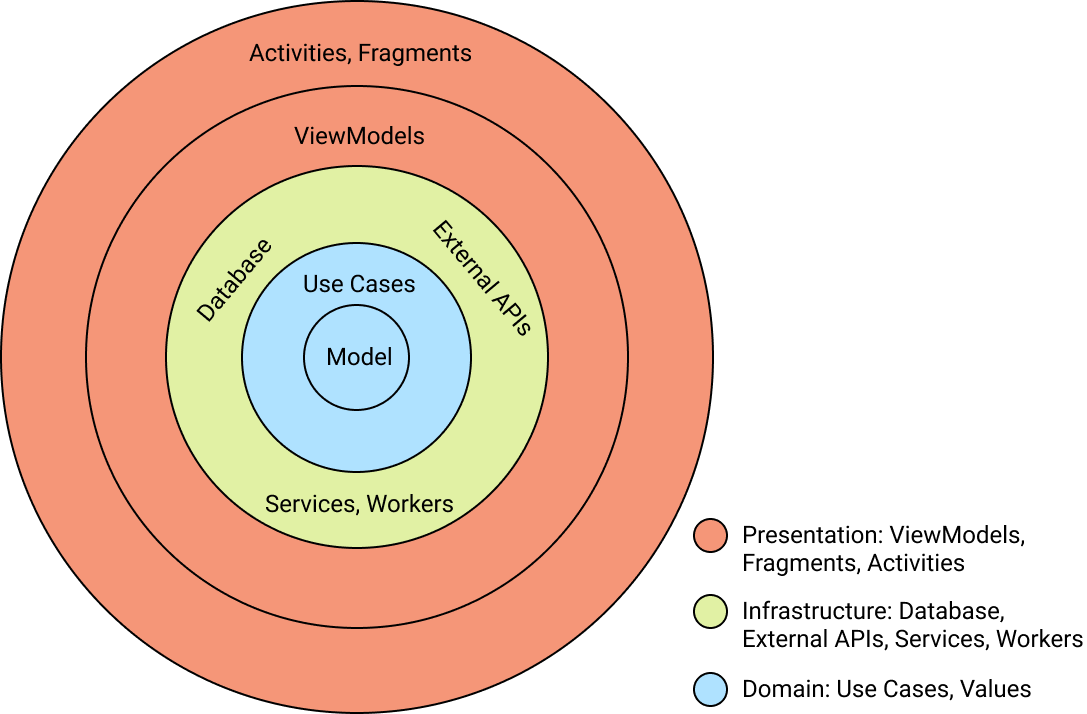
\includegraphics[width=0.465\textwidth]{Architecture.png}
  \caption{Nivelurile conceptuale ale arhitecturii aplicației
  \label{fig:arhitectura}}
\end{figure}

O caracteristică importantă a arhitecturii este aceea că abstractizarea descrește din centru înspre margini. Dependințele în cadrul acesteia sunt orientate către centru. Astfel, un nivel mai abstract nu depinde de un detaliu, ci invers, detaliile depind de abstractizări. Această caracteristică se realizează urmând principiul inversării dependințelor. Pentru a inversa dependințele, un nivel mai înalt definește o interfață care este implementată la un nivel inferior. Această interfață este injectată mai apoi în componenta ce necesită un serviciu implementat la un nivel inferior. Injectarea dependințelor este exemplificată în programul \ref{lst:diExample}.

\lstinputlisting[
  style=javaCodeStyle, 
  caption={ReceiptsUseCaseImpl.kt}, 
  label=lst:diExample
  ]{./code/DiExample.kt}

La nivelul unui \emph{usecase} este necesar accesul la baza de date. Dar la acest nivel detaliul implementării bazei de date nu este relevant. Aceasta poate fi \emph{SQL} sau o simplă colecție în memorie. De aceea este definită interfața \texttt{ReceiptsRepository} care apoi este implementată la nivelul \emph{infrastructure}.

Metoda recomandată pentru injectarea dependințelor în Android este librăria \emph{Dagger 2}. Dacă majoritatea librăriilor pentru injectarea dependințelor utilizează reflexia la \emph{run-time}, Dagger folosește anotările definite în pachetul \texttt{javax.inject} pentru a genera cod la \emph{compile-time}. Avantajul acestei abordări este performanța sporită, dar are dezavantajul necesității de configurare din partea programatorului.

\section{Persistență}

Această aplicație folosește trei medii de persistență pentru stocarea datelor:

\begin{itemize}
\item
  \textbf{sqlite}: datele textuale aferente bonurilor;
\item
  \textbf{internal storage}: imaginile aferente bonurilor;
\item
  \textbf{shared preferences}: datele predefinite și alte configurații;
\end{itemize}

\subsection{SQLITE}\label{sqlite}

Aceasta este o bază de date relațională ce este preinstalată pe sistemul de operare Android. Modelul de date stocat în această bază de date este unul simplu, prezentat în Figura \ref{sqldata}. Aceste tabele sunt generate cu ajutorul librăriei \emph{Room}, folosind codul de mai jos:

\begin{figure}[!ht]
    \centering
    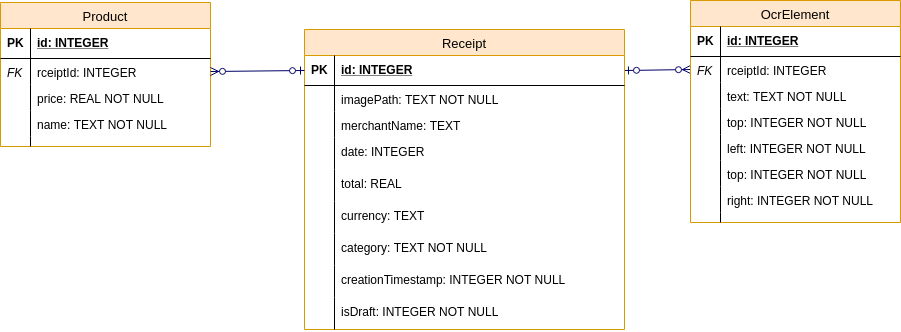
\includegraphics[width=\textwidth]{./figures/ReceiptScanDb.png}
    \caption{Modelul de date SQL \label{sqldata}}
\end{figure}

% \lstinputlisting[style=javaCodeStyle, caption=Entities.kt]{./code/Entities.kt}

\subsection{Spațiul de stocare intern}

Pe spațiul de stocare intern sunt salvate imaginile aferente bonurilor, fiind inaccesibile altor aplicații. Acestea sunt salvate sub un nume aleatoriu, care este salvat în tabela sql (proprietatea imagePath din tabela Receipt).

\subsection{Shared Preferences} \label{technical:sharedPreferences}

\emph{Shared preferences} sunt niște fișiere xml accesibile aplicațiilor Android, unde acestea pot salva valori sub format cheie-valoare. Aici sunt stocate:

\begin{itemize}
    \item
    categoria predefinită pentru bonuri;
    \item
    moneda predefinită;
    \item
    permite sau nu colectarea anonimă a bonurilor;
    \item
    un id unic al aplicației, generat la instalare;
\end{itemize}



    \chapter{Detalii și implementare}\label{implementation}

Secțiunile precedente au prezentat specificațiile aplicației, arhitectura și principalele tehnologii care facilitează implementarea. În continuare vor fi discutate detaliile de implementare ale fiecărei funcționalități.

\section{Algoritmul de extragere a informației}

Înțelegerea conținutului bonurilor fiscale din imagini reprezintă principala provocare a acestui proiect și funcționalitatea în jurul căreia este construită întreaga aplicație. În mod natural, aceasta se desparte în două sarcini:

\begin{itemize}
  \item 
  Recunoașterea textului;
  \item
  Extragerea informațiilor din textul neprocesat;
\end{itemize}

Metode mai bune pentru a rezolva această provocare pot ține cont de imagini și pentru a doua sarcină și pot folosi metode mai avansate, de \emph{machine learning}, pe măsură ce sunt colectate mai multe date. Aceste opțiuni sunt subiectul unor cercetări viitoare.

\subsection{Recunoașterea textului}

O constrângere pentru rezolvarea acestei sarcini este aceea ca procesarea să se facă pe dispozitiv. Astfel, datele utilizatorului nu părăsesc dispozitivul decât cu acordul său.

O soluție \emph{open source} populară pentru rezolvarea problemelor OCR este \emph{Tesseract} \cite{Tesseract}. Pentru dezvoltatorii de aplicații mobile, Google oferă librăria \emph{Firebase Vision}, cu suport gratuit pentru OCR pe dispozitiv. Comparația dintre cele două soluții a fost făcută astfel:

\begin{itemize}
  \item 
  Firebase Vision a fost rulat folosind un test de instrumentare, întrucât această librărie nu poate rula decâ pe un dispozitiv mobil;
  \item
  Tesseract a fost rulat pe un computerul personal, folosind \emph{Python};
  \item
  Imaginea a fost preprocesată doar pentru Tesseract, întrucât această librărie nu oferă o performanț satisfăcătoare pe imagini neprocesate;
  \item
  Preprocesarea a constat în aplicarea unui algoritm care să elimine fundalul, să transforme imaginea î alb-negru și să uniformizeze luminozitatea;
  \item
  Asupra ambelor rezultate a fost aplicat un algoritm care să grupeze chenarele de text pe linii;
  \item 
  Metrica după care au fost comparate cele două soluții este cea a acurateții textului recunoscut;
  \item 
  Cele două script-uri folosite pentru a rula cele două soluții se găsesc în anexa \ref{apx:Anexa1}.
\end{itemize}

În urma a mai multor teste, am observat că \emph{Tesseract} este mai susceptibil la zgomot și nu oferă rezultate de aceeași calitate ca \emph{Firebase Vision}. Un exemplu ușor este imaginea \ref{fig:exampleReceipt}. Textele extrase de cele două soluții sunt prezentate în figura \ref{fig:ocrResults}, unde se vede cantitatea de zgomot mai ridicată în rezultatul obținut cu \emph{Tesseract}. De asemenea, \emph{Tesseract} a emis alte câteva caractere non-utf8 de zgomot, ce nu au putut fi redate în acest text. De menționat este și efortul necesar pentru a integra \emph{Tesseract} într-o aplicație mobilă. În același timp, \emph{Firebase Vision} este disponibilă ca o dependință \emph{gradle}.

\begin{figure}[hb]
  \centering
  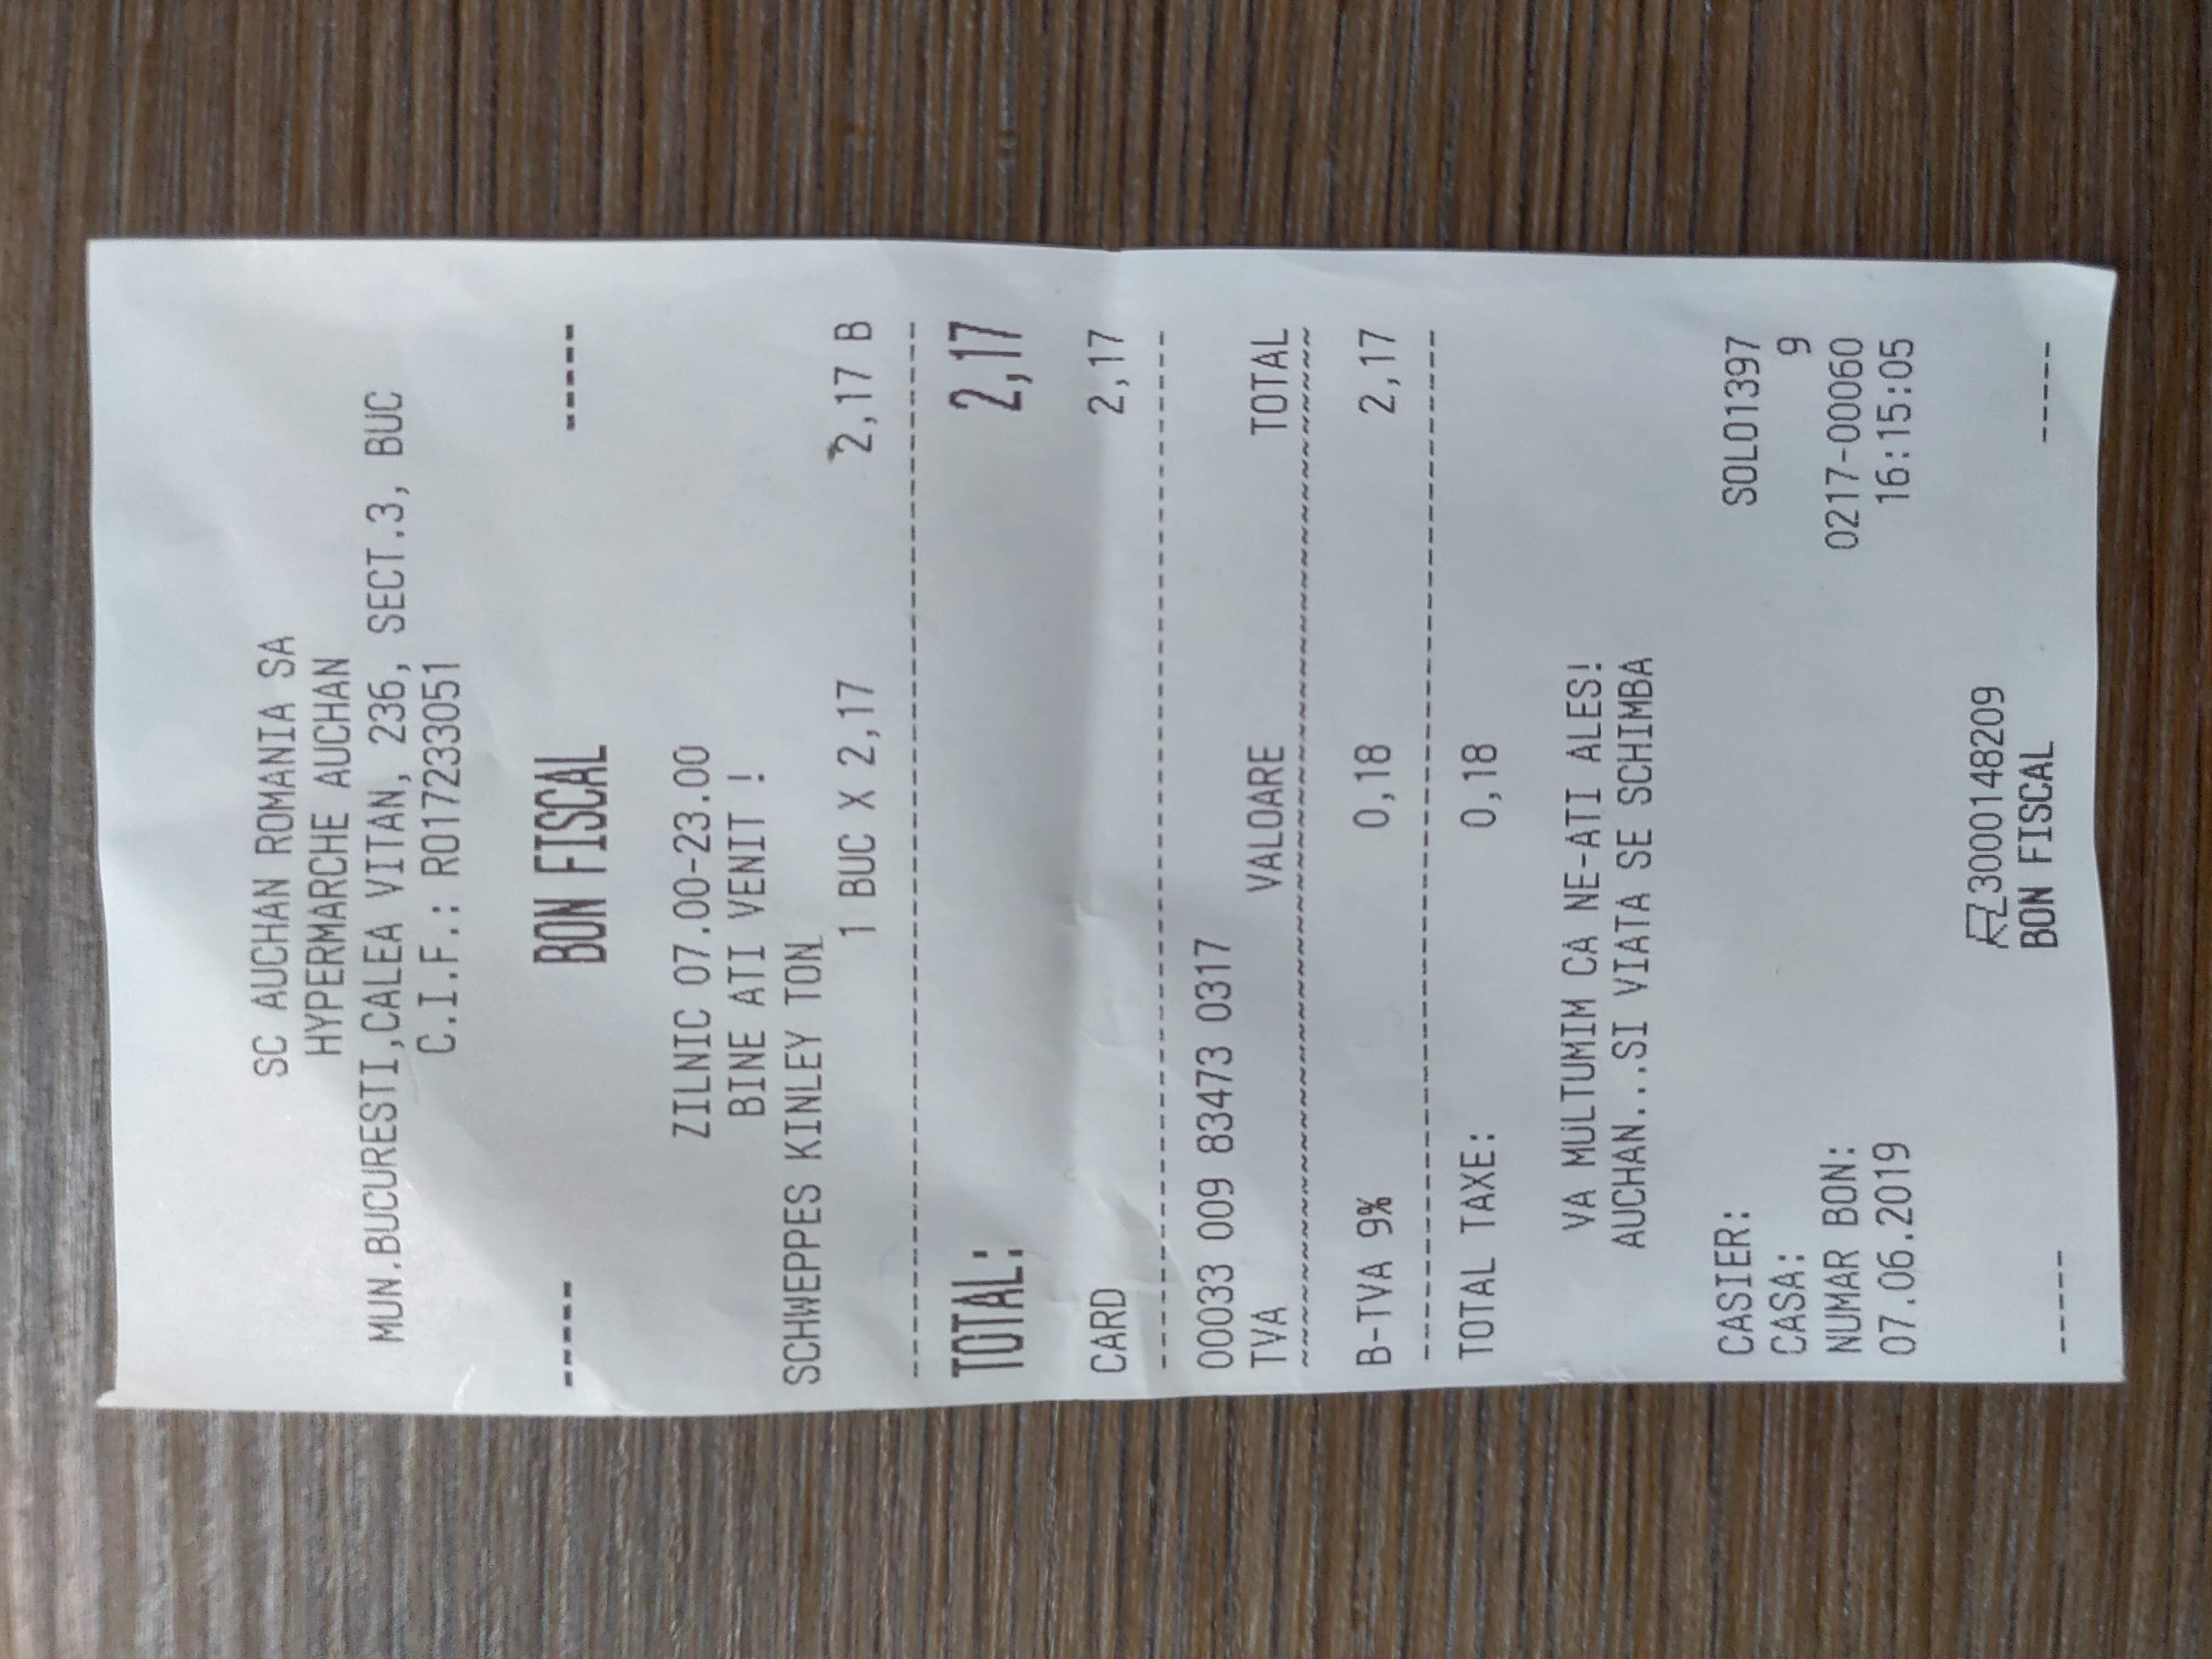
\includegraphics[width=0.5\textwidth,angle=-90]{receipt.jpg}
  \caption{Exemplu bon}
  \label{fig:exampleReceipt}
\end{figure}

\begin{figure}
  \begin{subfigure}{0.48\textwidth}
  \lstinputlisting[frame=single,breaklines=true,autogobble]{./samples/firebaseVisionOcrResult.txt}
  \caption{Firebase Vision OCR result}
  \label{fig:firebaseResult}
  \end{subfigure}
  \hfill
  \begin{subfigure}{0.48\textwidth}
  \lstinputlisting[frame=single,breaklines=true,autogobble]{./samples/tesseractOcrResult.txt}
  \caption{Tesseract OCR Result}
  \label{fig:tesseractResult}
  \end{subfigure}
  \caption{Textul extras de cele două soluții OCR}
  \label{fig:ocrResults}
\end{figure}

Performanța superioară a \emph{Firebase Vision} ar fi suficientă pentru a alege această librărie. La aceasta se adaugă și ușurința integrării și lipsa necesității de preprocesare. Dezavantajul major al acestei librării este integrarea unui serviciu extern, care nu este open source în codul aplicației, dar acesta nu este unul foarte mare pentru versiunea curentă a aplicației. Așadar, pentru sarcina de OCR am ales soluția \emph{Firebase Vision}.

\subsection{Extragerea informațiilor din text}

Procesarea textului rezultat în urma procesului de OCR se face pe baza unor reguli observate în majoritatea bonurilor fiscale. Firebase Vision returnează textul și chenarele de text, grupate în blocuri, linii și elemente, în funcție de coordonatele geometrice din imagine. Această organizare pe blocuri nu este de folos în procesarea de față, dar organizarea pe linii este, din moment ce informația din bonurile fiscale este așezată în format cheie-valoare, pe linii. De aceea, prima etapă în extragerea informațiilor este renunțarea la structura de blocuri și organizarea în linii raportate la întregul document. Această etapă se face după algoritmul:

\begin{enumerate}
  \item
  Extrage liniile din blocuri;
  \item
  Sortează liniile de sus în jos, în funcție de punctul lor de mijloc; Consideră liniile ca fiind elementele OCR;
  \item
  Grupează elementele OCR după distanța relativă dintre punctele lor de mijloc: elementele la o distanță mai mică de jumătate din media înălțimii tuturor elementelor se află în același grup;
\end{enumerate}

Implementarea acestui algoritm se găsește în Anexa \ref{apx:Anexa2}. Acest proces este ilustrat și în figura \ref{fig:ocrProcessing}. Organizarea la nivel de \textbf{bloc} este reprezentată în albastru, cea de \textbf{linie} în verde, iar cea de \textbf{element} în roșu. Se observă ca în organizarea dorită se renunță la structurile de blocuri, liniile se extind pe toată lățimea bonului, iar elementele devin fostele linii.

\begin{figure}[ht]
  \centering
  \begin{subfigure}{0.49\textwidth}
    \centering
    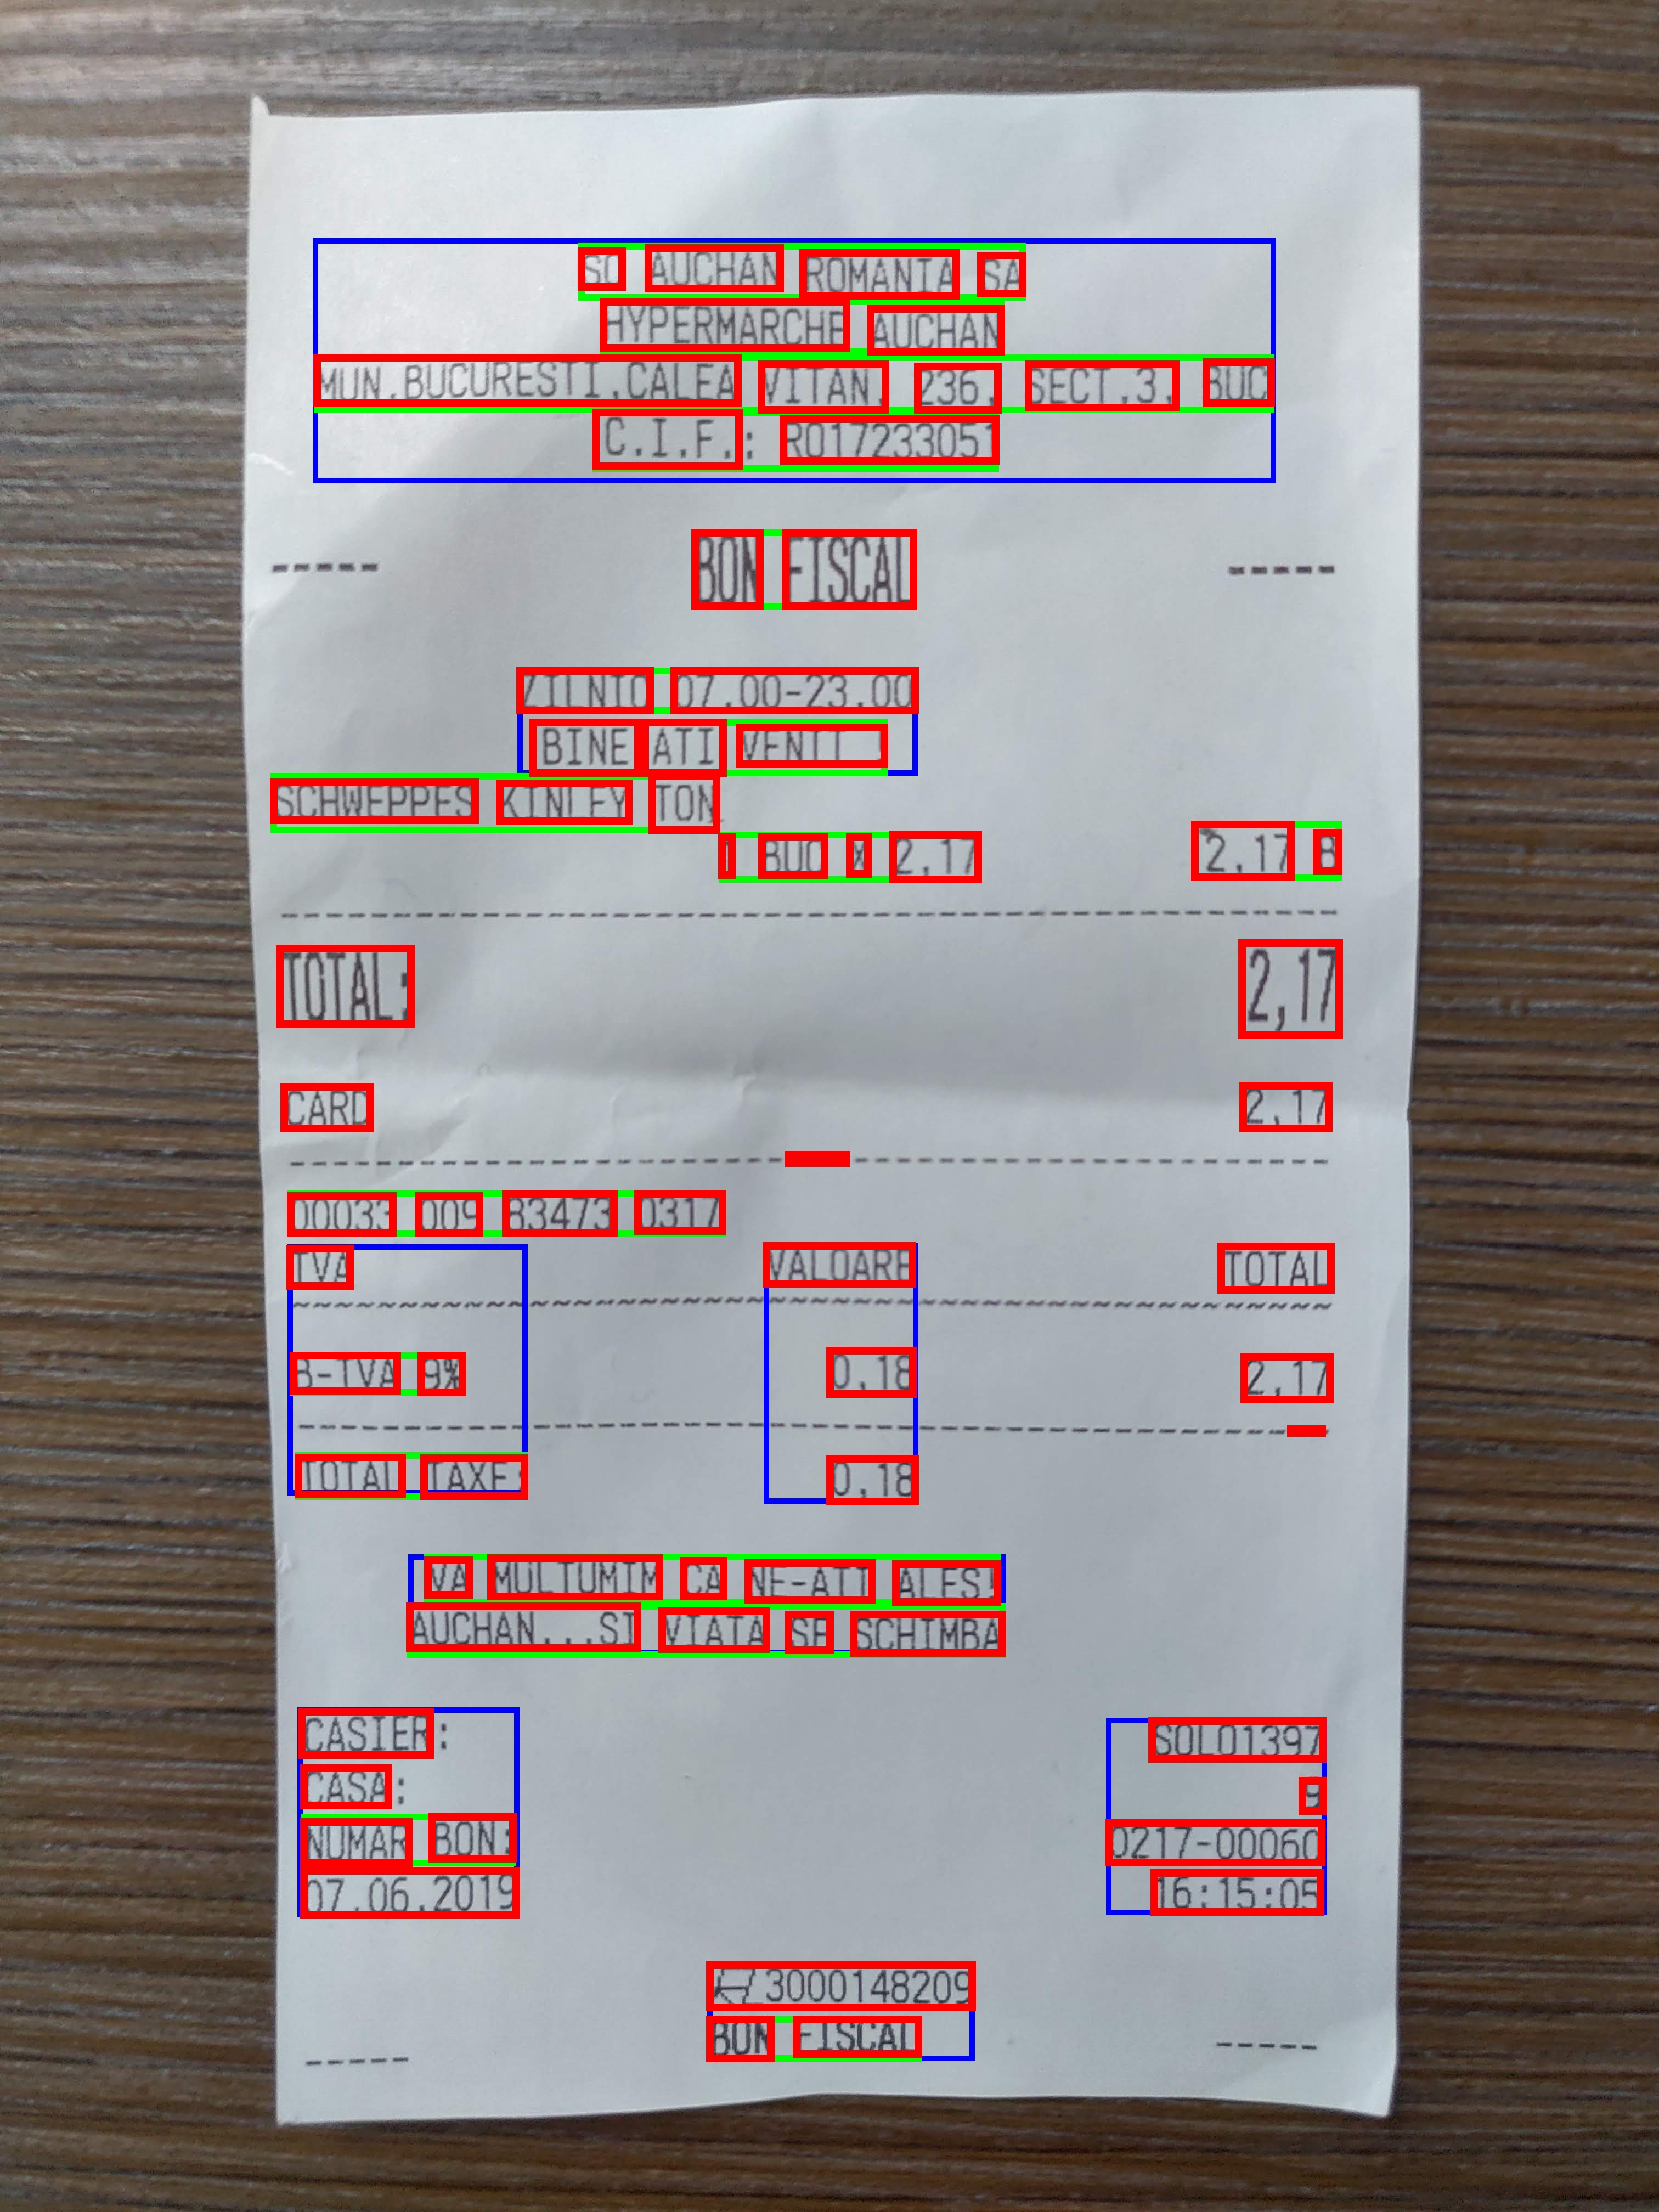
\includegraphics[width=5.5cm]{fibBlocks.jpg}
    \caption{Organizarea rezultatului OCR}
    \label{fig:ocrOutputBoxes}
  \end{subfigure}
  \begin{subfigure}{0.49\textwidth}
    \centering
    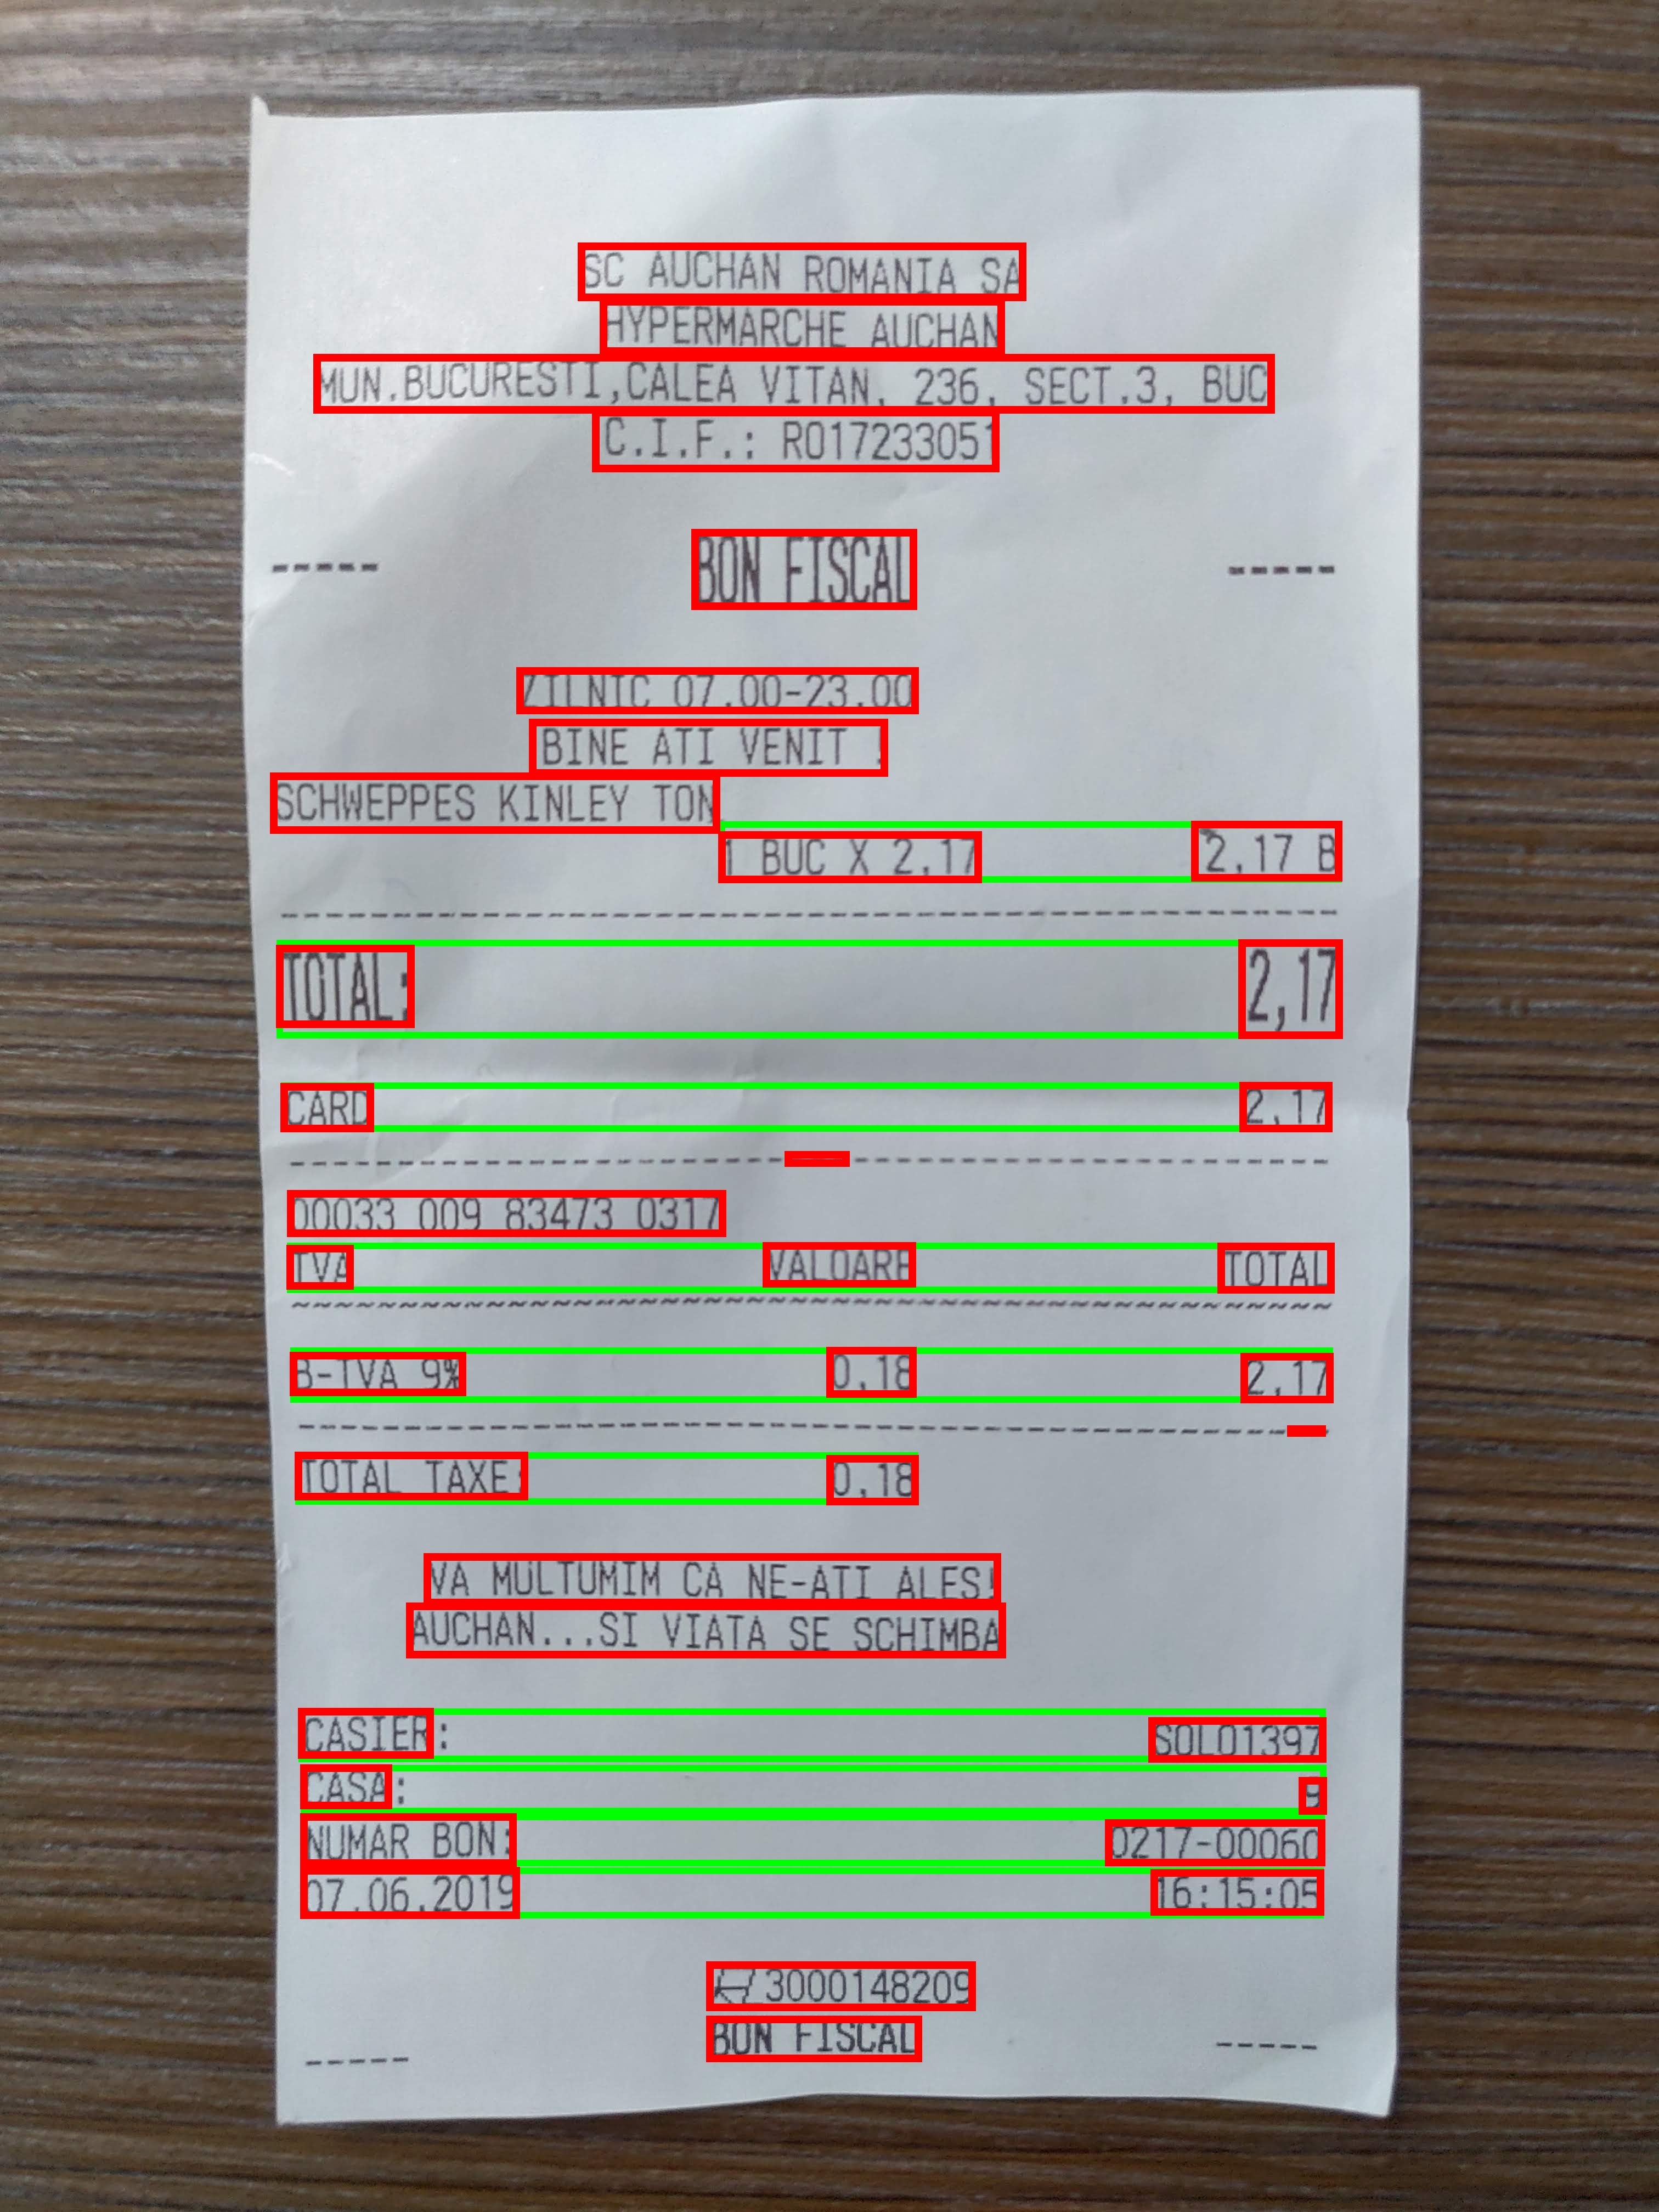
\includegraphics[width=5.5cm]{myBlocks.jpg}
    \caption{Organizarea elementelor OCR dorită}
    \label{fig:desiredBoxes}
  \end{subfigure}
  \caption{Procesul de organizare a rezultatului OCR}
  \label{fig:ocrProcessing}
\end{figure}

Având textul din imagine organizat în grupuri de cuvinte apropiate (vechile linii returnate de \emph{Firebase Vision}) și linii raportate la întreaga imagine, ordonate de sus în jos, informațiile relevante sunt extrase după următoarele reguli:

\begin{itemize}
  \item
  \textbf{Numele comerciantului}:
  \begin{enumerate}
      \item
      Extrage prima linie. Dacă aceasta este formată dintr-o singură literă, continuă extragerea. Această regulă este motivată de faptul că multe bonuri pot conține la început un logo ce poate fi confundat cu o literă.
      \item
      Dacă linia curentă are înălțimea peste media tuturor liniilor, atunci verifică următoarea linie. Dacă și aceasta are înălțimea peste medie și mai puțin de 3 cuvinte, consideră numele comerciantului ca fiind concatenarea celor două linii. În caz contrar, consideră numele comerciantului ca fiind textul liniei curente.
  \end{enumerate}
  \item
  \textbf{Data achiziției}: aplică o serie de expresii regulate pentru a parsa date din întregul text. Dacă sunt găsite mai multe date, alege data cea mai apropiată de data curentă. Dacă nu este găsită nicio dată, consideră data curentă.
  \item
  \textbf{Produse și preț total}: Acestea sunt procesate parcurgând liniile de sus în jos și alcătuind o listă obiecte de tip cheie-valoare. Cheile sunt nume de produse sau cuvinte cheie care să marcheze prețul total, iar valorile sunt prețuri, numere fracționare. Produsele și prețurile aferente sunt considerate toate obiectele care sunt întâlnite deasupra primului obiect ce marchează totalul.
  \item
  \textbf{Categoria și moneda}: aceste valori sunt citite din setările predefinite și pot fi modificate de utilizator.
  \textbf{Categoria și moneda}: aceste valori sunt citite din setările predefinite și pot fi modificate de utilizator.
  \textbf{Categoria și moneda}: aceste valori sunt citite din setările predefinite și pot fi modificate de utilizator.
  \textbf{Categoria și moneda}: aceste valori sunt citite din setările predefinite și pot fi modificate de utilizator.
\end{itemize}

Implementarea detaliată a algoritmului de extragere a informațiilor este prezentat în Anexa \ref{apx:Apendix3}.



\section{Capturarea și înțelegerea imaginilor}

La nivelul domeniului, algoritmul de OCR este ascuns sub interfața \texttt{Scannable}, care este implementată la nivelul infrastructurii. Aceasta expune două metode, \texttt{ocrElements()} și \texttt{image()}, ce furnizează elementele textuale și imaginea sub abstractizarea \texttt{Observable} din RxJava.

\lstinputlisting[style=javaCodeStyle, caption=Interfețele Scannable și ExtractUseCase]{./code/ScannableExtractUseCase.kt}

\texttt{ExtractUseCase} modelează și orchestrează funcționalitățile aferente ecranului de scanare:

\begin{itemize}
  \item 
  Valoarea \texttt{preview} expune un flux de elemente OCR care să fie afișate pe ecran, deasupra camerei, pentru a ajuta utilizatorul în capturarea imaginii;

  \item
  Funcția \texttt{fetchPreview} permite livrarea unui nou cadru surprins de cameră, care să fie procesat asincron, iar rezultatul să fie livrat către \texttt{preview};

  \item
  Funcția \texttt{extract} declanșează procesarea imaginii bonului și salvarea informațiilor în baza de date, returnând id-ul entității salvate;

  \item
  Valoarea \texttt{state} marchează daca o imagine este procesată pentru extragerea unui bon sau nu, sau dacă a fost întâmpinată o eroare;
\end{itemize}

Procesarea unei imagini durează în funcție de performanțele telefonului, timp de câteva secunde. Părăsirea ecranului de scanare este permisă în acest timp deoarece obiectul \texttt{ExtractUseCase} nu este distrus odată cu obiectul vizual, ceea ce nu întrerupe procesarea.

Pentru implementarea vizorului am folosit librăria \emph{CameraView}\cite{CameraView}. O constrângere a acesteia este aceea că imaginea surprinsă este pusă automat pe un \emph{thread} secundar și este accesată printr-un \emph{callback}. Această abordare intră în conflict utilizarea \emph{RxJava}. La o inspecție a codului acestei librării am observat existența unei metode \emph{package private} de a obține imaginea capturată în mod \emph{sincron}. Așadar, într-un modul nou am implementat decoratorul \texttt{RxPictureResult} în pachetul librăriei, care să expună imaginea capturată într-un \texttt{Observable}.

Procesarea cadrelor pentru a afișa în timp real textul recunoscut de modului \emph{OCR} este limitată la maxim 15 cadre pe secundă pentru a nu suprasolicita dispozitivul. \emph{CameraView} livrează cadre la o rezoluție scăzută pentru procesarea în timp real, ceea ce scade timpul de procesare al acestora, dar si calitatea textului extras. Aceasta nu este o problemă deoarece afișarea în timp real are doar rolul de a ghida utilizatorul. Dacă o porțiune de text este recunoscută la o rezoluție scăzută, atunci aceasta va fi recunoscută și în imaginea capturată la rezoluție întreagă. Pentru afișarea chenarelor am implementat obiectul vizual \texttt{OcrOverlay}, care este așezat deasupra vizorului.



\section{Gestionare Drafturi}

\subsection{Implementare}

La nivelul modelului, aceste opțiuni sunt reprezentate prin interfața \texttt{DraftsUseCase}. Atât funcționalitatea de listare, cât și cea de editare se folosesc de funcționalitatea \emph{Room} prin care atunci când apare o modificare la nivelul bazei de date, o nouă valoare este emisă pentru interogările deja executate. Astfel, este ușoară o implementare reactivă pentru aceste funcționalități.

\lstinputlisting[style=javaCodeStyle, caption=Interfața Drafts Use Case]{./code/DraftsUseCase.kt}

Editarea câmpurilor text se face în manieră \emph{on the fly}, ceea ce înseamnă că nu este necesar un ecran separat drept formular și apăsarea unui buton de persistare a modificărilor. Aceasta se realizează înregistrând un \emph{callback} pe câmpurile de text, care apelează funcția de update. Această abordare ridică problema unor fluxuri de date mult prea rapide. De aceea, asupra fluxului de modificări este aplicat operatorul RxJava \texttt{throttleLast}. Figura \ref{fig:throttle}, din documentația RxJava \cite{ThrottleLast} ilustrează modul în care acest operator funcționează.

\begin{figure}[h]
  \centering
  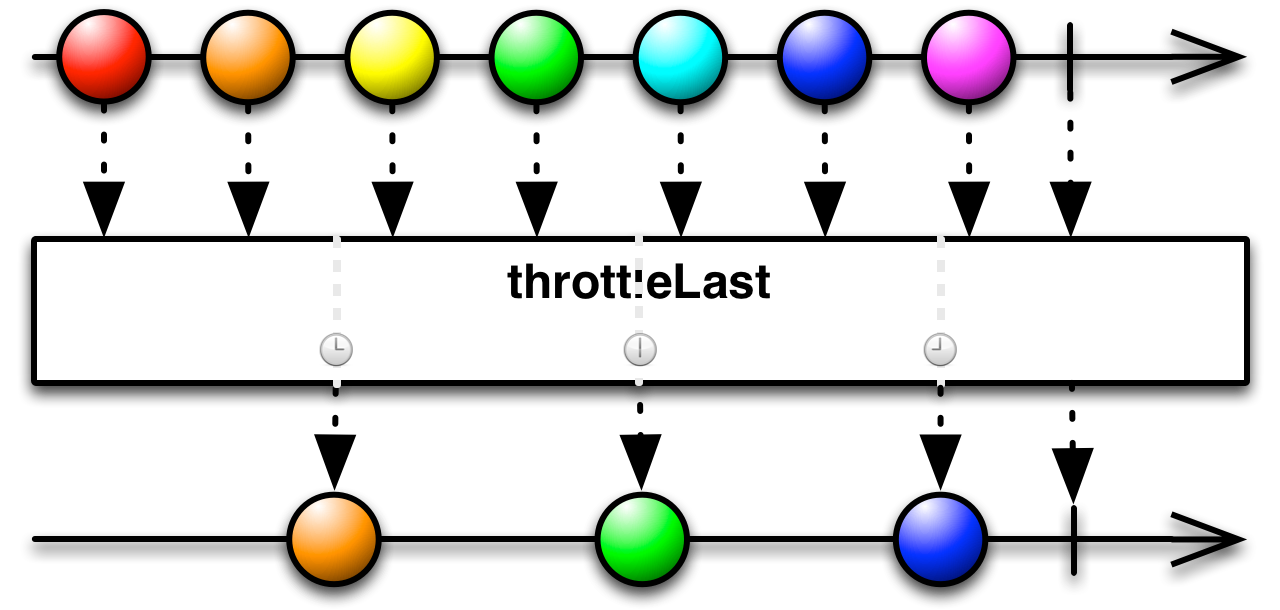
\includegraphics[width=0.7\textwidth]{throttleLast.png}
  \caption{Ilustrație throttleLast}
  \label{fig:throttle}
\end{figure}

În continuare este prezentată utilizarea operatorului \texttt{throttleLast}, împreună cu un exemplu de utilizare. Funcția \texttt{throttled} primește argumentele pentru aplicarea operatorului și o funcție și returnează o nouă funcție care are aceeași signatură, același comportament, dar executată la o rată de timp specificată. În acest mod sunt exemplificate funcțiile de ordin înalt și abilitatea de a reprezenta funcțiile ca valori în limbajul Kotlin.

\lstinputlisting[style=javaCodeStyle, caption=Funcții throttled]{./code/ThrottleImplementation.kt}

\section{Setări}

% Ecranul de setări controlează valorile predefinite utilizate în extragerea datelor despre bonuri și indicatorul care permite sau nu colectarea datelor. Modificarea acestor valori nu este inclusă explicit în domeniul aplicației, de aceea această funcționalitate este implementată numai la nivelul prezentării și infrastructurii. Interfețele definite de model, \texttt{CollectingOption} și \texttt{ReceiptDefaults} sunt implementate de clasa \texttt{PreferencesDao}, care este folosită pentru a accesa mediul de stocare \texttt{SharedPreferences}. 

% \begin{figure}[h]
%   \centering
%   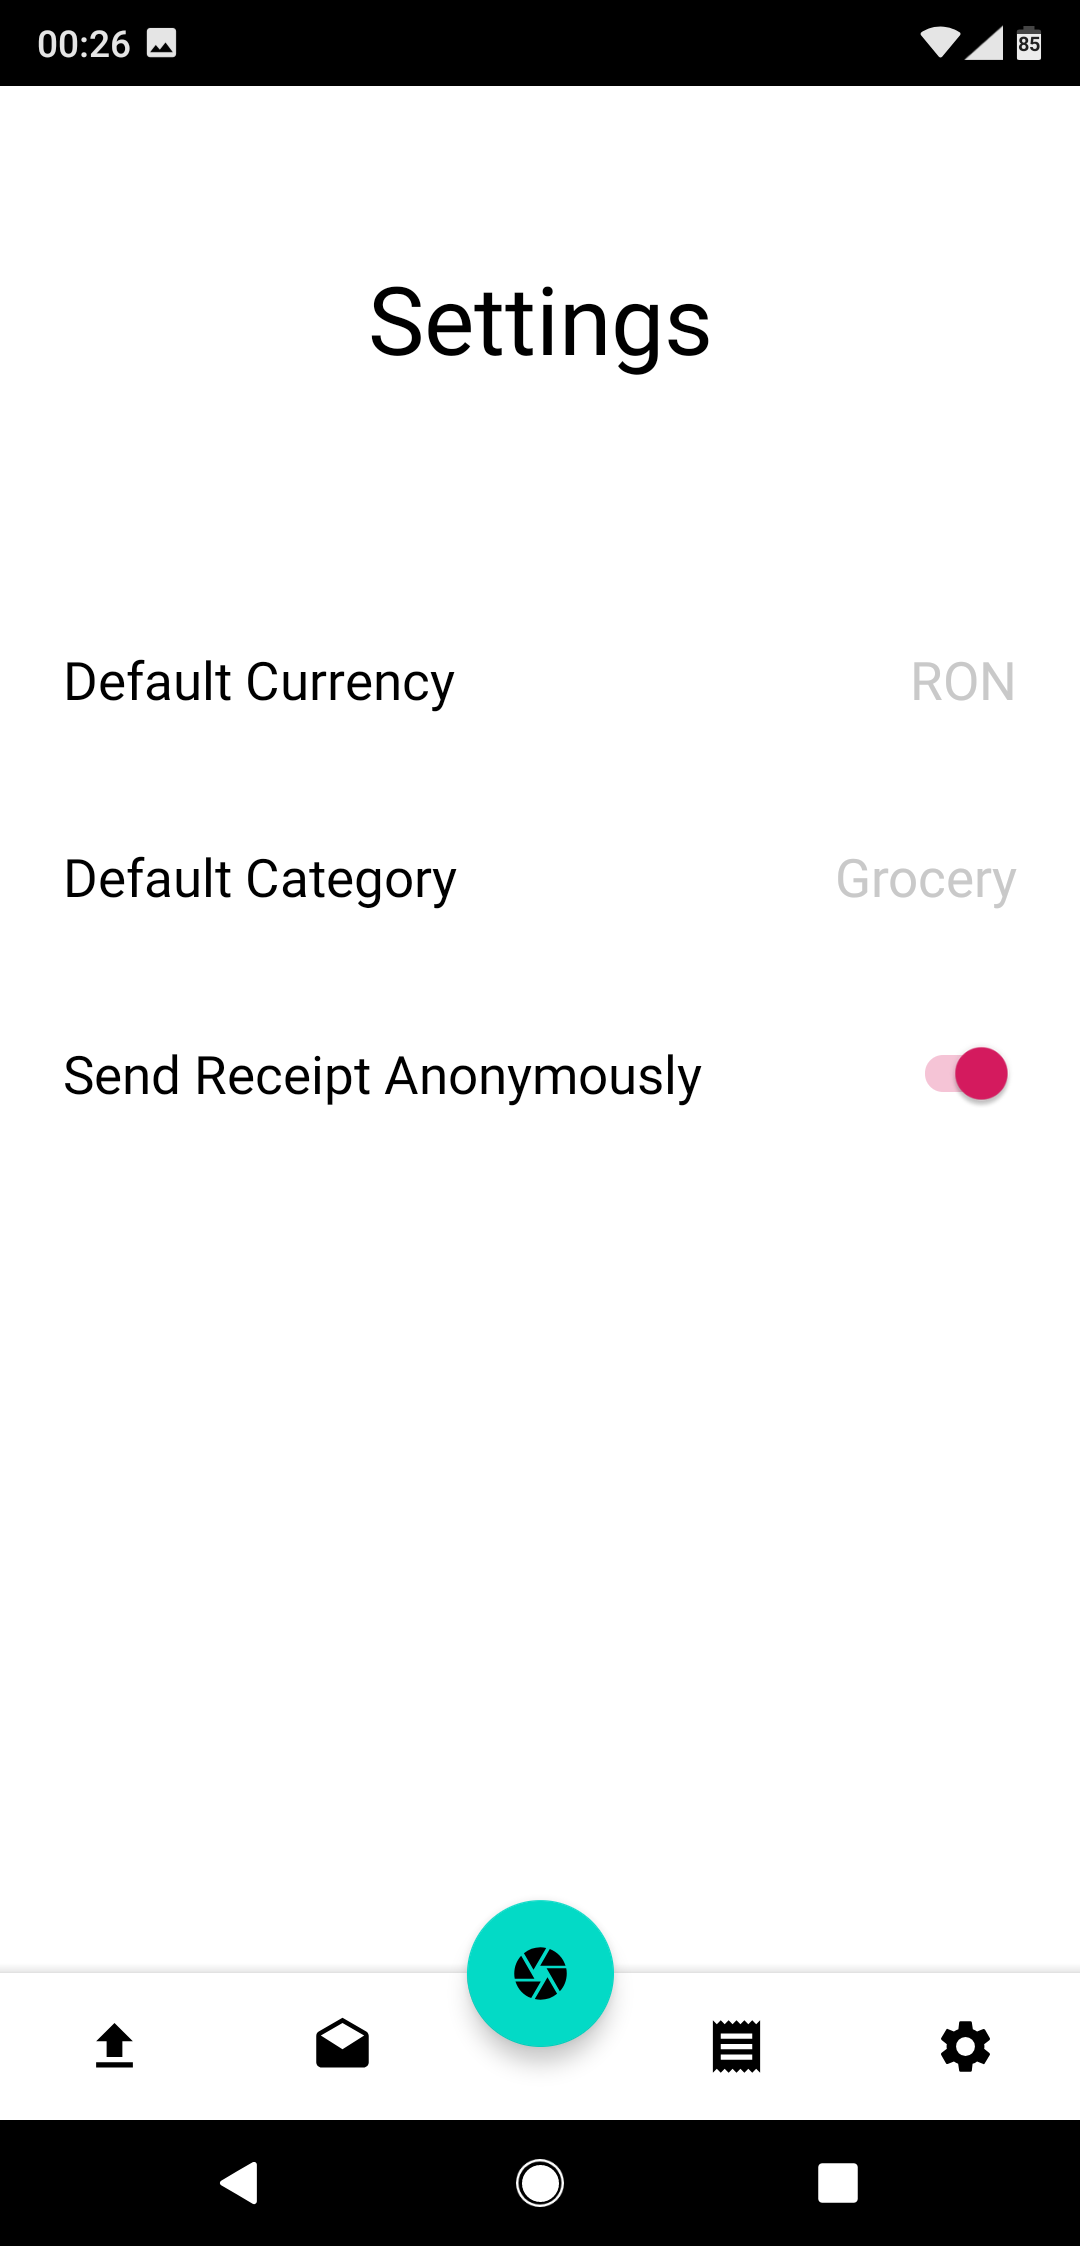
\includegraphics[width=\screenwidth]{SettingsScreen.png}
%   \caption{Ecranul de setări}
%   \label{settingsScreen}
% \end{figure}
\section{Colectarea Datelor}

La nivelul domeniului, funcționalitatea de colectare de date are o reprezentare simplă, dată de interfața \texttt{ReceiptCollector}. Atunci când \texttt{DraftsUseCase.Manage::moveToValid} se execută cu succes, metoda \texttt{send} este apelată și aceasta declanșează procesul de colectare a bonului curent.

\lstinputlisting[style=javaCodeStyle, caption={Interfața ReceiptCollector}, label={lst:receiptCollector}]{./code/ReceiptCollector.kt}

Constrângerea acestei funcționalități de a avea un impact minim asupra experienței utilizatorului este rezolvată prin implementarea acesteia ca \texttt{Worker}, ceea ce permite executarea întârziată, în \emph{background} și sub anumite condiții. Din moment ce această acțiune nu este critică pentru utilizator, ea se execută numai atunci când dispozitivul este conectat la o rețea \emph{UNMETERED} (Wi-Fi).

Worker-ul primește ca parametru id-ul bonului care trebuie sincronizat în cloud. La instanțiere, îi sunt injectate un obiect de acces la baza de date și opțiunea de colectare, așa cum este prezentată în programul \ref{lst:settingsInterfaces}. Dacă această opțiune este activată, bonul este extras din baza de date și trimis în cloud, împreună cu imaginea aferentă.

Așa cum este specificat, colectarea se face în mod anonim. Totuși, un identificator care să arate dacă anumite date provin de la același dispozitiv poate fi util. De aceea bonurile sunt trimise împreună cu un \emph{UUID}. Acest identificator este generat prima dată când este cerut și salvat în \emph{shared preferences}. De menționat este că acest identificator nu supraviețuiește la reinstalarea aplicației.

Această funcționalitate, la fel ca cea de export, utilizează serviciile cloud \emph{Firebase}. Autentificarea se face pe baza cheii de aplicație generată din consola \emph{Firebase} atunci când aplicația este atașată unui proiect. Această cheie este salvată în fișierul \emph{google-services.json} și distribuită împreună cu aplicația.

Stocarea datelor textuale se face în colecția \emph{collected} din \emph{Firebase Firestore}, iar imaginile se stochează în \emph{Firebase Cloud Storage}, în directorul \emph{collected}.

\section{Export}

\subsection{Implementare}

La nivelul domeniului, funcționalitatea de export este modelată de interfața \texttt{ExportUseCase}. Aceasta definește funcțiile de listare a tuturor exporturilor de pe dispozitiv, creeare a unui nou export și marcarea unui export ca finalizat la primirea unei notificări.

\lstinputlisting[style=javaCodeStyle, caption=Interfața ExportUseCase]{./code/ExportUseCase.kt}

Trimiterea datelor către cloud se face printr-un serviciu de tipul \emph{foreground}. Pe sistemul Android, \emph{serviciile foreground} sunt servicii care interacționează cu utilizatorul prin intermediul unei notificări și au șanse foarte mici de a fi oprite de către sistem pentru a recupera resurse. Acestea sunt recomandate pentru a executa activități de lungă durată care nu blochează interfața și care sunt declanșate de o acțiune a utilizatorului. Funcția \texttt{upload} este apelată într-un astfel de serviciu cu argumentul obținut pe baza formularului prezentat mai sus. La creearea argumentului \texttt{Session} este generat un id unic ce va fi folosit pentru identificarea exportului pe durata funcționării acestuia.

Interacțiunea aplicației cu serviciile cloud Firebase pentru această funcționalitate este ilustrată în diagrama din figura \ref{exportProcess}.

\begin{figure}[ht]
  \centering
  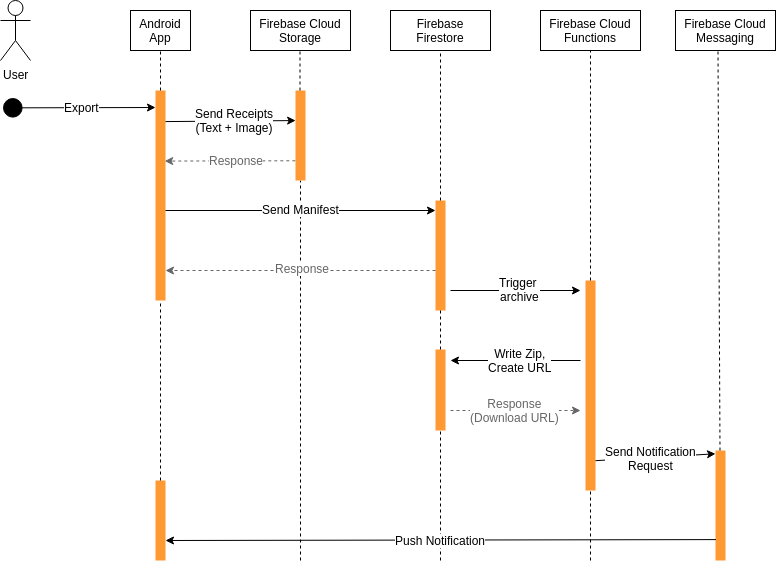
\includegraphics[width=\textwidth]{ExportSequence.png}
  \caption{Procesul de trimitere}
  \label{exportProcess}
\end{figure}

Serviciul de \emph{foreground} încarcă bonurile aferente exportului într-un spațiu de stocare \emph{Firebase Cloud Storage}, sub un folder ce are numele id-ului unic generat, în format JSON (opțional și imaginile JPEG respective). La încărcarea cu succes a acestor fișiere, obiectul \texttt{Session} este trimis ca manifest în colecția \emph{manifests} din serviciul \emph{Firebase Firestore}.

O funcție \emph{Firebase Cloud Functions} este configurată pentru a asculta modificări ale colecției \emph{manifests} și a se declanșa la creearea unui nou obiect. Aceasta citește id-ul manifestului și opțiunea de format (JSON sau CSV) și procesează fișierele din folder-ul corespunzător din \emph{Cloud Storage}. Apoi încarcă o arhivă \emph{zip} a acestui folder în folder-ul \emph{downloads} din Cloud Sotrage și generează un link de descărcare, pe care îl trimite către serviciul \emph{Firebase Cloud Messaging} pentru a fi trimis mai departe ca notificare către dispozitiv.

Pentru ca notificarea să ajungă doar la dispozitivul care a creeat exportul, aplicația folosește clientul Android al \emph{Firebase Cloud Messaging}. Acesta presupune implementarea unui serviciu ce extinde \texttt{FirebaseMessagingService}. Acest serviciu generează un \emph{token} folosit pentru a primi notificări și îl face disponibil în metoda \texttt{onNewToken(token:\ String)}. Aplicația salvează acest token în \emph{shared preferences} și îl trimite în obiectul manifest. Astfel, acest token ajunge pe cloud, de unde este transmis către \emph{Firebase Cloud Messaging}.

\emph{Firebase Cloud Messaging} suportă două tipuri de mesaje: \emph{notification messages} și \emph{data messages}, sau o combinație dintre cele două. (Firebase n.d.) Pentru ca notificarea să fie gestionată imediat ce a fost primită în metoda \texttt{onMessageReceived(message:\ RemoteMessage)} a serviciului \texttt{FirebaseMessagingService} este folosită doar funcționalitatea de \emph{data message}. Odată ce notificarea este recepționată de către dispozitiv, metoda \texttt{markAsFinished(notification:\ FinishedNotification)} este apelată pentru a actualiza baza de date și o notificare este afișată.



    \chapter*{Concluzii}\label{conclusions}
\addcontentsline{toc}{chapter}{Concluzii}  

Am gândit \AppName{} în jurul ideii democratizării informațiilor financiare. Utilizarea bonurilor fiscale ca date de intrare pentru aplicație aduce avantajul de a nu depinde de modul în care a fost făcută achiziția. Majoritatea utilizatorilor au mai multe carduri, dar folosesc și bani lichizi pentru unele achiziții. Soluția propusă adună toate aceste tranzacții într-un singur loc.

Un alt avantaj este flexibilitatea datelor. Soluția propusă oferă o vizualizare rapidă a tranzacțiilor în aplicație, asemenea altor soluții, dar oferă și exportul datelor, pentru ca acestea să fie folosite pentru analize detaliate în programe cum ar fi \emph{Excel}.

Principalul obstacol întâmpinat în dezvoltarea aplicației a fost înțelegerea automată a bonurilor fiscale. Abordarea aleasă are două mari dezavantaje. Primul este acela că performanța ei este limitată de performanța modulului \emph{OCR} ales. Al doilea dezavantaj este lipsa flexibilității și mai ales imposibilitatea ca extragerea informațiilor să se îmbunătățească fără a face modificări în codul aplicației.

Funcționalitatea de export o găsesc foarte utilă pentru urmărirea cheltuielilor personale. Câteva întrebări la care se poate răspunde având la îndemână nu doar lista tranzacțiilor, ci și produsele de pe fiecare chitanță sunt: \emph{Ce sumă am cheltuit în această lună pe apă, pâine etc.?}, \emph{Cu cât sunt mai scumpe produsele la supermarket-ul X comparativ cu Y?}. De asemenea, aceste date sunt și o înregistrare a evoluției prețurilor de-a lungul timpului. Adunarea acestor date manual este o sarcină laborioasă, pe care puțini o fac. \AppName este o unealtă care să faciliteze această sarcină.

Din punct de vedere al implementării, limbajul \emph{Kotlin} aduce o experiență de dezvoltare mult mai plăcută comparativ cu \emph{Java 7}. Librăriile din cadrul \emph{Android Architecture Components} încearcă să ofere soluții moderne pentru structurarea și implementarea aplicațiilor. Totuși, menținerea compatibilității cu versiunile vechi ale \emph{API}-urilor \emph{Android} limitează gradul de dezvoltare al acestora. Un \emph{bug} rezolvat recent care evidențiază această problemă este păstrarea subscribției unui fragment la un \emph{viewModel} după ce acest fragment și-a încheiat ciclul de viață, ceea ce conduce la \emph{memory leaks}. Privind retrospectiv, poate că \emph{Flutter}, un \emph{framework} mult mai nou, dezvoltat în limbajul \emph{Dart} ar fi fost o alegere mai bună pentru implementarea acestei aplicații.

O experiență plăcută am avut lucrând cu \emph{RxJava}. Această librărie are o complexitate ridicată și necesită un efort considerabil din partea programatorului pentru a o înțelege. Avantajul primit în schimb este ușurința cu care se poate executa cod asincron. De asemenea, abordarea funcțională a acestei librării face testarea mai ușoară și reduce din posibilele \emph{bug-uri}.

Dezvoltarea ulterioară a acestei aplicații vizează publicarea acesteia și promovarea pe medii online, cum ar fi \emph{Reddit} sau \emph{ProductHunt}. De asemenea, această aplicație este în mod \emph{open source} și poate aduna contribuții de la mai mulți programatori, care pot îmbunătăți metoda de extragere a informațiilor din chitanțe.

    
    \printbibliography[title=Bibliografie]

    \begin{appendices}
    \chapter{Script-urile folosite pentru compararea soluțiilor OCR}\label{apx:Anexa1}

Codul testului rulat pentru a obține textul din \ref{fig:firebaseResult}:

\lstinputlisting[style=javaCodeStyle, caption=LineUnification.kt]{./code/firebaseVisionOcr.kt}

Script-ul rulat pentru a obține textul din \ref{fig:tesseractResult}:

\lstinputlisting[style=javaCodeStyle, caption=LineUnification.kt]{./code/tesseractOcr.py}

    \chapter{Algoritmul de unificare a liniilor}\label{apx:Anexa2}

\lstinputlisting[style=javaCodeStyle, caption=LineUnification.kt]{./code/LineUnification.kt}


    \chapter{Algoritmul de extragere a informațiilor}\label{apx:Apendix3}

\lstinputlisting[style=javaCodeStyle, caption=Algoritmul de extragere]{./code/ExtractionAlgorithm.kt}

    \end{appendices}
    
\end{document}
